%%%%%%%%%%%%%%%%%%%%%%%%%%%%%%%%%%%%%%%%%%%%%%
%%% PREAMBLE
\documentclass[12pt, table]{beamer}
\usepackage{graphicx}
\graphicspath{{images/}}
\usepackage{rotating}
\usepackage{wasysym}
\usepackage[tone,extra]{tipa}
\usepackage{tabularx}
\usepackage{multirow}
\usepackage{qtree}
\usepackage[normalem]{ulem}
\usepackage{adjustbox} % to make figues and tables fit the boxes
\usepackage{float}
\usepackage{multimedia}
\usepackage{enumerate}
\usepackage{lmodern}
\usepackage{eurosym}
\usecolortheme[named=black]{structure}
\usepackage[ngerman]{babel}
\usepackage[T1]{fontenc}
\usepackage[absolute,overlay]{textpos} % for logo in header 
\usepackage{chngcntr}
% define bibliography style
\usepackage[round]{natbib}
\bibpunct{(}{)}{;}{a}{}{,}
\setcitestyle{notesep={: }} % replace comma with colon in citations
\usepackage{cite}

\usepackage{gb4e} % for examples
\newcolumntype{Y}{>{\centering\arraybackslash}X}
\newcommand{\myipa}[1]{{\shorthandoff{"}\scantokens{\tipaencoding#1\endinput}}}
%%%%%%%%%%%%%%%%%%%%%%%%%%%%%%%%%%%%%%%%%%%%%%
%%% define footline
\setbeamertemplate{footline}{
   \begin{beamercolorbox}[ht=4ex,leftskip=0.4cm,rightskip=.4cm]{author in head/foot}
    \hrule
    \vspace{0.1cm}
    \hfill \newline
    \insertshortauthor  \hfill \insertframenumber
        \vspace{0.2cm}
   \end{beamercolorbox}
   \vspace*{0.1cm}
} 

%%%%%%%%%%%%%%%%%%%%%%%%%%%%%%%%%%%%%%%%%%%%%%
%%% define headline
\setbeamertemplate{headline}
{
  \leavevmode%
  \hbox{%
  \begin{beamercolorbox}[wd=.8\paperwidth, ht=0.9cm, dp=0.2cm, left, rightskip=.2cm]{section in head/foot}%
    \usebeamerfont{subsection in head/foot} \hspace*{.1cm}

\includegraphics[height=0.8cm,width=0.8cm]{images/unilogo.png}
\insertshorttitle
  \end{beamercolorbox}%
  \begin{beamercolorbox}[wd=.5\paperwidth, ht=0.9cm, dp=0.2cm, right, leftskip=0cm]{subsection in head/foot}%
    \usebeamerfont{section in head/foot}\insertsectionhead\hspace*{0.2cm} 
  \end{beamercolorbox}}%
  \hrule
  \vskip0pt%
}
%%%%%%%%%%%%%%%%%%%%%%%%%%%%%%%%%%%%%%%%%%%%%%
%%%
%%%%%%%%%%%%%%%%%%%%%%%%%%%%%%%%%%%%%%%%%%%%%%
%%% START
\author{Martin Schweinberger}
\title{53-506 Introduction to English Linguistics}
\begin{document}
\begin{frame}[plain]
\titlepage
\begin{center}
SS 2015\\
\end{center}    
%Figure 1
\begin{figure}[H]
\centering
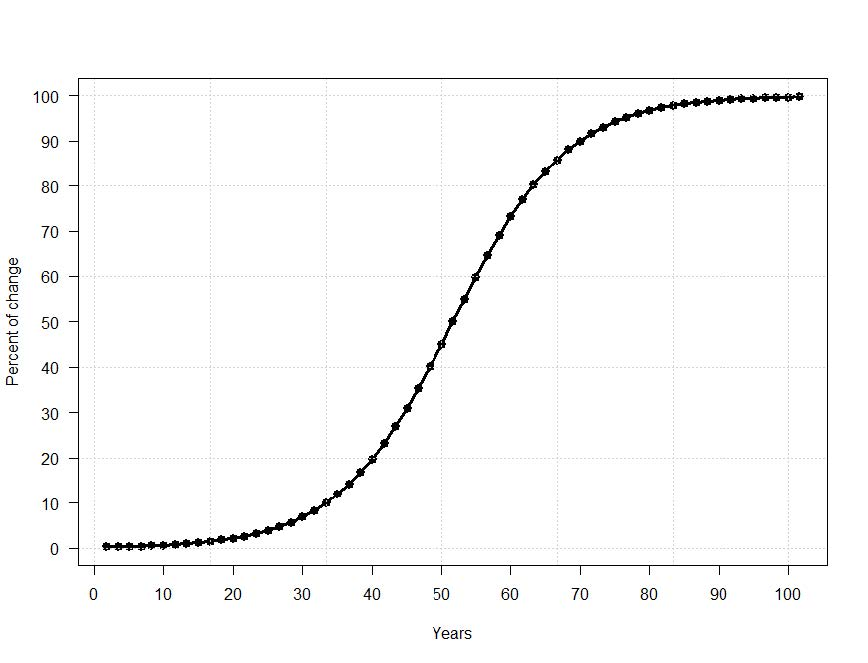
\includegraphics[scale=0.3]{fig1.png} 
\label{fig:fig1}
\end{figure}
\end{frame}

%%%%%%%%%%%%%%%%%%%%%%%%%%%%%%%%%%%%%%%%%%%%%%
%%% Overview

\section{Overview}
%%% Overview
\begin{frame}
\frametitle{Overview}
\begin{center}
\adjustbox{max height=\dimexpr\textheight\relax,
max width=\textwidth}{
\begin{tabular}{l rr}
\multicolumn{2}{c}{}\\
Seminar Ia & 2h Friday 14-16 (+ 2h Tutorial)\\
Phil G & AA-E1, ENG-1, AA1, LAA1, LAA14 & \\
\hline
Martin Schweinberger & martin.schweinberger@uni-hamburg.de\\
Office and office hours & 1169, Thursday 16-17\\
\hline
Sabrina Sarkodie-Gyan & sabrina.sarkodie@student.uni-hamburg.de\\
Monday 14-16 & Von-Melle-Park 6, 701\\
\hline 
Britta Stuhl & britta.stuhl@student.uni-hamburg.de\\
Tuesday 12-14 & Von-Melle-Park 6, 1172
\end{tabular}
}
\end{center}
\end{frame}

%%% Overview
\begin{frame}
\frametitle{Overview}
Course description\\
\begin{itemize} 
\item This course will introduce students to the basic concepts and methods in the study and description of language. We shall be looking at the basic levels of linguistic analysis such as phonetics and phonology, morphology, syntax, semantics and pragmatics. We will also be looking into where these overlap and briefly address where linguistics cuts into other academic disciplines. The course will be taught in English.
\end{itemize}
\end{frame}

%%% Overview
\begin{frame}
\frametitle{Attendence}
\begin{itemize} 
\item You are allowed to miss two classes.
\item If you miss only 2 classes, you do not need an excuse because you are officially allowed to miss 15\% of a course!(cf. Modulhandbuch).
\item If you miss more than 2 classes, you have to contact me!
\item To pass this course you need to be present and participate regularly, and you have to pass the final exam.
\end{itemize}
\end{frame}

\begin{frame}
\frametitle{Overview}
Tutorials\\
\begin{itemize}
\item The tutorials help you understand the course content and will prepare you for the final exam. So: go to one of the tutorials!
\end{itemize}
Exercise/ work sheets \dots
\begin{itemize}
\item will NOT be graded or corrected
\item will also help you understand the course content and will prepare you for the final exam.
\end{itemize}
\end{frame}

\begin{frame}
\frametitle{Overview}
Tipps
\begin{itemize}
\item Martin Hilpert (a linguist who also studied English Linguistics at Hamburg University) uploaded his videos showing his lecture $"$Intro to  English linguistics$"$ to YouTube (I highly recommend it(!): \footnotesize{https://www.youtube.com/playlist?list=PLKgdsSsfw-fYCJ90tLikJRbXvl74g6FUw}
\end{itemize}
Literature
\begin{itemize}
\item The literature serves as a guide BUT what counts is what I teach here in class and what is in the materials I designed for this course(!). 
\item Introductory books I recommend are \citet{berg2013intro}, \citet{meyer2010introducing}, \citet{fromkin2013introduction}, and \citet{kortmann2001linguistik}.
\end{itemize}
\end{frame}

\begin{frame}
\begin{center}
\frametitle{Overview}
\adjustbox{max height=\textheight,
max width=\textwidth}{
\begin{tabular}{l l}
\hline
\multicolumn{2}{c}{\textbf{Levels of linguistic analysis}}\\
\hline
Semiotics & study of signs\\
Phonetics & study of sounds\\
Phonology & study of sound systems and interaction\\
Morphology & study of word structure\\
Syntax & study of sentence structure\\
Semantics & study of meaning\\
\hline
Pragmatics & study of meaning in context\\
Sociolinguistics/Language Change & study of variation in language\\
Psycho-linguistics & study of language and mind/brain\\
\hline
\end{tabular}
}
\end{center}
\end{frame}

%%% course plan
\begin{frame}
\begin{center}
\frametitle{Overview}
\adjustbox{max height=\textheight,
max width=\textwidth}{
\begin{tabular}{l ll}
\hline
\textbf{Session}  & \textbf{Date}  & \textbf{Topic} \\
\hline
1  & Fr, 10. Apr. 2014  & Formalities and overview\\
2  & Fr, 17. Apr. 2014  & Language and the Brain\\
3  & Fr, 24. Apr. 2014  & History of the English Language\\
4  & Fr, 8. May 2014  & Phonetics: Phones and Phonemes\\
5  & Fr, 15. May 2014  & no class (Phonology: Allophony and Syllables)\\
6  & Fr, 22. May 2014  & Morphology: Building Meaningful Blocks\\
7  & Fr, 5. Jun. 2014  & Syntax: Word Classes and Phrases\\
8  & Fr, 12. Jun. 2014  & Syntax: Sentence Structure and Semantic Roles\\
9  & Fr, 19. Jun. 2014  & Semantics: The Classical View\\
10  & Fr, 26. Jun. 2014  & Semantics: Prototypes and Categorization\\
11  & Fr, 3. Jul. 2015  & Pragmatics: Language in the Real World\\
12  & Fr, 10. Jul. 2015  & In-class exam\\
\hline
\end{tabular}
}
\end{center}
\end{frame}

\begin{frame}
\frametitle{ }
\begin{center}
Overview Microlinguistics\\
\end{center}
\end{frame}

\begin{frame}
\frametitle{Phonetics and Phonology}
\begin{tabularx}{\textwidth}{l l}
Phonetics: & study of sounds\\
Phonology: & study of sound systems and sound interaction\\
\end{tabularx}
\begin{itemize}
\item How do we produce sounds?\\
\begin{itemize}
\item \textipa{pr@\textsecstress n2nsI\textprimstress eISn}\\
$<$pronunciation$>$
\item \textipa{lO:$^{r}$nO:d@}\\
$<$law and order$>$ (sounds like 'Laura Norder')
\item Dialect refers to differences on all levels of grammar, i.e. lexicon, morphology, syntax.
\end{itemize}
\item What makes someone sound "German"?
\end{itemize}
\end{frame}

\begin{frame}
\frametitle{Morphology}
Morphology is the study of word structure\\
\begin{itemize}
\item What is a word?
\item Sehirlilestiremediklerimizdensiniz.
\end{itemize}
\begin{exe}
\ex 
\gll Sehir- li- les- tir- eme- dik- ler- imiz- den- siniz\\
town- s/o.from become cause.to can't whom those we one.of you.are\\
\trans You are one of those whom we can't turn into a town-dweller (Deutscher 2005: 24)
\end{exe}
\begin{itemize}
\item Internal structure, e.g. disgraceful: dis\#grace\#ful\\
\item Word formation: How do we "form" (new) words?
\end{itemize}
\end{frame}

\begin{frame}
\frametitle{Syntax}
Syntax is the study of sentence structure\\
\begin{itemize}
\item How do we combine words?
\begin{exe}
\ex I like apples and bananas.
\ex ?Apples I like and bananas.
\ex *Like bananas apples I and.
\end{exe}
\item Lexical and structural ambiguity:
\begin{exe}
\ex She saw the man with the binoculars.
\ex Time flies like an arrow. Fruit flies like a banana.
\end{exe}
\end{itemize}
\end{frame}

\begin{frame}
\frametitle{Syntax}
\footnotesize{\Tree [.S [.NP [.N She ] ] [.VP [.V saw ] [.NP [.A the ] [.N man ] [.PP [.P with ] [.NP [.N binoculars ] ] ] ] ] ]}
\end{frame}

\begin{frame}
\frametitle{Syntax}
\footnotesize{\Tree [.S [.NP [.N She ] ] [.VP [.V saw ] [.NP [.A the ] [.N man ] ] [.PP [.P with ] [.NP [.N binoculars ] ] ] ] ]}
\end{frame}

\begin{frame}
\frametitle{Semantics}
Semantics is the study of meaning (relationships)\\
Features versus Prototypes
\begin{itemize}
\item Name 3 birds.
\item Name 3 tools.
\item Name 3 colors.
\end{itemize}
\end{frame}

\begin{frame}
\frametitle{Semantics}
Semantics is the study of meaning (relationships)\\
Features versus Prototypes
\begin{itemize}
\item Name 3 birds.
\item Name 3 tools.
\item Name 3 colors.
\end{itemize}
All of you had sparrow/pigeon, hammer/screwdriver, or red/blue.
\end{frame}

\begin{frame}
\frametitle{Pragmatics (not microlinguistics)}
Pragmatics is the study of meaning in context\\
What is meant by what is said?
\begin{itemize}
\item Can you take out the trash.
\item It's warm in here.
\item I wouldn't do that.
\end{itemize}
In all three cases, the literal meaning deviates from the intended message.
\end{frame}

%%%%%%%%%%%%%%%%%%%%%%%%%%%%%%%%%%%%%%%%%%%%%%
%%% Overview
\section{Semiotics}
\begin{frame}
\frametitle{What is Language?}
Discuss in groups of three:
\begin{itemize}
\item What is Language/a language?
\item Language vs. dialect vs. accent?
\item Provide a brief definition for each.
\item How many languages are there? 
\end{itemize}
\begin{textblock*}{1.5cm}(6cm,1.2cm)
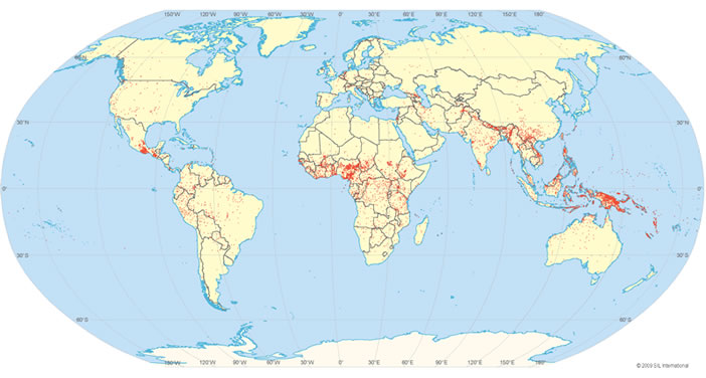
\includegraphics[width=5.5cm]{images/worldlanguages.png}
\end{textblock*}
\end{frame}

\begin{frame}
\frametitle{What is Language?}
Discuss in groups of three:
\begin{itemize}
\item What is Language/\\ a language?
\begin{itemize}
\item Continuum, hard to separate!
\end{itemize}
\item Language vs. dialect vs. accent?
\begin{itemize}
\item Accent refers to differences in pronunciation, only.
\end{itemize}
\item Provide a brief definition for each.
\begin{itemize}
\item Dialect refers to differences on all levels of grammar, i.e. lexicon, morphology, syntax.
\end{itemize}
\item How many languages are there? 
\begin{itemize}
\item App. 6,000 (depending on what counts as a $"$language$"$)
\end{itemize}
\end{itemize}
\begin{textblock*}{1.5cm}(6cm,1.2cm)
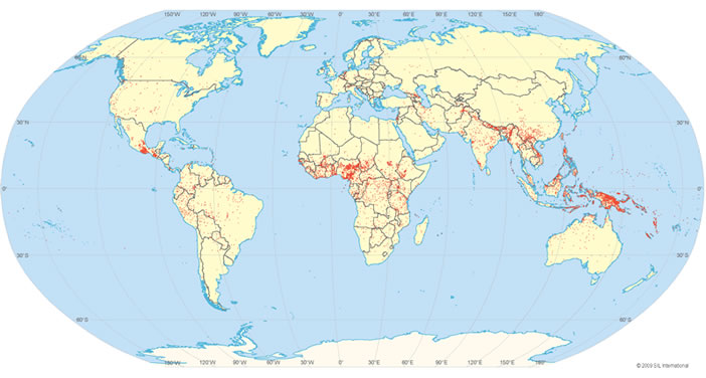
\includegraphics[width=5.5cm]{images/worldlanguages.png}
\end{textblock*}
\end{frame}

\begin{frame}
\frametitle{What is Language?}
Language is a system of visual, auditory, or tactile symbols (arbitrary signs) used in human communication and the rules used to manipulate them.\\
\begin{itemize} 
\item Human language differs from animal communication.
\item Only humans use language.
\item All human cultures use language. 
\item Every child learns language.
\item Language is handled by certain parts of the brain.
\item All languages share certain features.
\item All languages have certain regularities (grammar: word order).\\
\dots
\end{itemize}
\end{frame}

\begin{frame}
\frametitle{What is Language?}
Language is a system of visual, auditory, or tactile symbols (arbitrary signs) used in human communication and the rules used to manipulate them.\\
\begin{itemize} 
\item Language is social.
\item Language always changes.
\item All languages are related. 
\item Language is creative.\\
\dots
\end{itemize}
\end{frame}

%%% table of contents frame
\AtBeginSection[]
{
\begin{frame}
\frametitle{Table of Contents}
\tableofcontents[currentsection]
\end{frame}
}
%%% semiotics
\begin{frame}
\frametitle{Language and Communication}
Human language vs. animal communication\\
\begin{itemize}
\item But don't animals communicate too?
\item What is so different about human communication? 
\item How do we differentiate between a dog's bark, a bee dance and human communication?
\item Kanzi! 
\end{itemize}
\end{frame}

\begin{frame}
\movie[width=4cm]{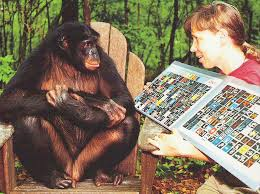
\includegraphics[width=10cm]{images/kanzi.jpg}}{movies/kanzisentences.avi}
\end{frame}

\begin{frame}
\frametitle{Features of Language}
\begin{itemize}
\item Displacement
\begin{itemize}
\item Momentary and immediate meaning $\neq$ ability to refer to past and/or future. (bee communication?)
\end{itemize}
\item Arbitrariness
\begin{itemize}
\item Usually no natural connection between a linguistic form and its meaning. Relation is arbitrary (willk{\"u}rlich), not iconic. (onomatopoeia? kikiriki)
\end{itemize}
\item Productivity
\begin{itemize}
\item Humans are frequently creating new expressions to refer to novel experiences, objects, or events. (bees: cannot communicate vertical distance).
\end{itemize}
\end{itemize}
\end{frame}

%%% semiotics
\begin{frame}
\frametitle{Features of Language}
\begin{itemize}
\item Traditional transmission
\begin{itemize}
\item Genetic acquisition and traditional transmission. 
\item Korean infant will speak English, if adopted by L1 English speakers.
\item Some animals are born with a distinct set of signals that they produce instinctively (cat: meow).
\end{itemize}
\item Duality
\begin{itemize}
\item Language is organized at two levels simultaneously. 
\item Level of physical production of distinct sounds and the level of meaning (interpreting combination of sounds).
\end{itemize}
\end{itemize}
\end{frame}

%%% Semiotics and Linguistics
\begin{frame}
\frametitle{Linguistics and Semiotics}
Linguistics\\ 
\begin{itemize} 
\item Linguistics is the scientific study of systems of symbols, i.e. of language or particular languages, and of their rules (grammar) used by humans to communicate and express ideas and feelings.
\end{itemize}
Semiotics\\ 
\begin{itemize} 
\item Semiotics is the scientific study of signs, sign systems of and sign processes in general, i.e. not restricted to verbal, human signs.
\end{itemize}
\end{frame}

%%% Semiotics and Linguistics
\begin{frame}
\frametitle{Semiotics and Signs}
Signs
\begin{itemize} 
\item A sign is sth. that stands for sth. else:\\
\textit{aliquid stat pro aliquo} 
\item Form
\begin{itemize} 
\item Sound pattern, gesture, picture, writing,\\fashion, hair cut, \dots
\end{itemize}
\item Function
\begin{itemize} 
\item Meaning, concept, mental representation
\end{itemize}
\end{itemize}
\begin{textblock*}{2cm}(9cm,1.5cm)
\includegraphics[width=2cm]{images/hair.png}
\end{textblock*}
\begin{textblock*}{3cm}(10cm,5.5cm)
\includegraphics[width=2cm]{images/traffic.png}
\end{textblock*}
\begin{textblock*}{6cm}(6cm,2cm)
\includegraphics[width=2cm]{images/trafficlight.png}
\end{textblock*}
\begin{textblock*}{8cm}(8cm,7.5cm)
\includegraphics[width=2cm]{images/book.png}
\end{textblock*}
\begin{textblock*}{6cm}(3cm,8cm)
\textit{I will be here tomorrow.}
\end{textblock*}
\end{frame}

%%% Semiotics and Linguistics
\begin{frame}
\frametitle{Types of Signs}
Indexes ("pointing towards")
\begin{itemize}
\item Here, there, I, him, that\dots etc.\\
(note: there is still a symbolic/conventional element: ich, moi, lui etc.)
\end{itemize}
Icons (similarity)
\begin{itemize}
\item Onomatopoeia ("Lautmalerei")\\
E.g. \textit{splash}, \textit{crash}, \textit{swoosh}; \textit{that movie was so boooooring}.
\item These are very rare examples and context- and culture-specific.
\end{itemize}
Symbols (arbitrariness)
\begin{itemize}
\item Most of language is symbolic; i.e. conventionalized and has to be learned.
\end{itemize}
\end{frame}

%%% Additional frames
%%% semiotics
\begin{frame}
\frametitle{Saussure's sign}
\begin{itemize} 
\item Ferdinand de Saussure \\ (1857-1913; Swiss linguist)
\begin{itemize}
\item Contemporary linguistics is, to a \\ large extend, still based on \\ concepts developed by him.
\item His main ideas were published post \\ humously from his lecture materials \\ (1916) under the title \\ $"$Cours de linguistique g{\'e}n{\'e}rale$"$ (Course in General Linguistics).
\item He can be considered the founder of modern linguistics.
\item His school of thought is refered to as $"$ Structuralism$"$ (he is still an important figure in structuralist thought)
\end{itemize}
\end{itemize}
\begin{textblock*}{8cm}(9cm,1.5cm)
\includegraphics[width=3cm]{images/saussure.jpg}
\end{textblock*}
\end{frame}

\begin{frame}
\frametitle{Saussure's sign}
\begin{itemize} 
\item Ferdinand de Saussure \\ (1857-1913; Swiss linguist)
\begin{itemize}
\item Introduced the distinction between \dots
\begin{itemize}
\item Synchronic linguistics \\ (study of language at a certain time)
\item Diachronic linguistics \\(study of language change over time)
\end{itemize}
\item Introduced the $"$primacy of the spoken word$"$ 
\item Shift away from a purely diachronic perspective to a focus on synchronic language use.
\item Fostered the transition from the prescriptive period to descriptive approach towards language.
\end{itemize}
\end{itemize}
\begin{textblock*}{8cm}(9cm,1.5cm)
\includegraphics[width=3cm]{images/saussure.jpg}
\end{textblock*}
\end{frame}

\begin{frame}
\frametitle{Saussure's sign}
\begin{itemize} 
\item Ferdinand de Saussure \\ (1857-1913; Swiss linguist)
\begin{itemize}
\item Focus on the structure of language. 
\item Language system (langue) is the \\ center of study, not the concrete \\ language use (parole).
\item Principle of Arbitrariness\\[.2cm]
There is no internal link between a sound pattern and the meaning of a concept!\\[.2cm]
\item The concept of a dog is represented by different sound patterns depending on the linguistic code used to refer to a dog and, thus, depends upon social convention.
\end{itemize}
\end{itemize}
\begin{textblock*}{8cm}(9cm,1.5cm)
\includegraphics[width=3cm]{images/saussure.jpg}
\end{textblock*}
\end{frame}

\begin{frame}
\frametitle{Saussure's sign}
\begin{itemize} 
\item Ferdinand de Saussure (1857-1913; Swiss linguist)
\begin{itemize}
\item Each linguistic sign (word) consists out of a sound sequence (signifier) and a concept (signified)
\item The relationship between the sound sequence and the concept of a linguistic sign is arbitrary and depends upon social convention.\\
\includegraphics[width=6cm]{images/saussuresign.png}
\end{itemize}
\end{itemize}
\end{frame}

\begin{frame}
\frametitle{B{\"u}hler's $"$Organon Model$"$}
\begin{itemize} 
\item Karl B{\"u}hler (1879-1963) 
\begin{itemize}
\item approached language by \\ examining the (possible) \\ functions of language.
\item Father of $"$Functionalism$"$
\item The $"$Organon Model$"$ is a \\ functional description of \\ sign usage/communication.
\item Function(s) of language according to B{\"u}hler
\begin{itemize}
\item expressive function (express feelings/beliefs)
\item representative function (talk about the world)  
\item appellative function (e.g. make a request).
\end{itemize}
\begin{textblock*}{8cm}(8cm,1.5cm)
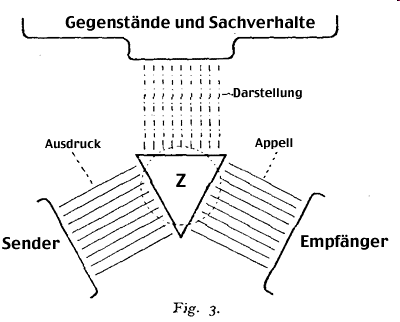
\includegraphics[width=4cm]{images/organon.png}
\end{textblock*}
\begin{textblock*}{8cm}(10.5cm,6cm)
\includegraphics[width=2cm]{images/buhler.jpg}
\end{textblock*}
\end{itemize}
\end{itemize}
\end{frame}

%%% table of contents frame
\AtBeginSection[]
{
\begin{frame}
\frametitle{Table of Contents}
\tableofcontents[currentsection]
\end{frame}
}

%%%%%%%%%%%%%%%%%%%%%%%%%%%%%%%%%%%%%%%%%%%%%%%%%%
%%% Language and the Brain

\section{Language and the Brain}
\begin{frame}
\frametitle{Introduction to English Linguistics}
\framesubtitle{Language and the Brain}
Today's topics and terms\\[.5cm]
\begin{itemize}
\item Aphasia
\item Language area
\item Critical period and plasticity 
\end{itemize}
\end{frame}

\begin{frame}
\frametitle{Language and the Brain}
Localizationism\\
\begin{itemize}
\item Brain consist of compartmentalized and specialized areas called  "modules"
\item Modules are specialized neurons in certain regions dealing with simpler tasks (e.g. exclusively language-related tasks)
\end{itemize}
Connectionism (holism)
\begin{itemize}
\item Language related abilities are carried out by larger parts of the brain
\item Focus on how language is dependent on other, broader cognitive abilities (memory, abstract thinking, attention,\dots)
\item No language centers but "network nodes"
\end{itemize}
\end{frame}

\begin{frame}
\frametitle{Localizationism}
\begin{itemize}
\item Paul Broca (1824-1880)
\item Brain has two hemispheres
\item $"$Damage to the left hemisphere \\ is more strongly correlated with language \\ impairment than damage to the right \\ hemisphere.$"$
\item Is there a language module \\ in the left hemisphere?
\end{itemize}
\begin{textblock*}{8cm}(9cm,1.3cm)
\includegraphics[width=3cm]{images/broca.png}
\end{textblock*}
\begin{textblock*}{8cm}(9cm,5cm)
\includegraphics[width=3cm]{images/brainslices.png}
\end{textblock*}
\end{frame}

\begin{frame}
\frametitle{Language impairments (aphasia)}
\begin{itemize}
\item Language deficits acquired after brain \\ injury.
\item Some aphasiacs perform normal on \\ non-verbal tests of IQ, they have neither trouble cooking, nor walking a complex route home. 
\item Aphasias are caused by damage to certain regions of the left hemisphere (language area)
Researchers discovered different kinds of aphasias 
\item Different symptoms correspond to different regions being impaired:
\begin{itemize}
\item more to the front: speech production.
\item more to the back: comprehension.
\end{itemize}
\end{itemize}
\begin{textblock*}{8cm}(9cm,1.5cm)
\includegraphics[width=3cm]{images/brocasarea.png}
\end{textblock*}
\end{frame}

\begin{frame}
\frametitle{Broca's aphasia}
\begin{itemize}
\item In 1861, Broca presented data from \\
 a patient called Tan Tan. Tan could \\ 
say this one syllable ($"$tan$"$) and \\ 
repeated it if asked to, but seemed \\ surprised that he couldn't get \\ his message across. Tan's comprehension was in fact good. 
\item Postmortem examination showed a brain lesion at the lower areas of the frontal lobe (Broca's region) 
\item Symptoms
\begin{itemize}
\item fluent, slow, deliberate, effortful, omission of grammatical markers (e.g. $"$Boy go store$"$ instead of $"$The boy has gone to the store$"$)
\end{itemize}
\end{itemize}
\begin{textblock*}{8cm}(8cm,1.5cm)
\includegraphics[width=4cm]{images/brainparts.png}
\end{textblock*}
\end{frame}

\begin{frame}
\frametitle{Wernicke's aphasia}
\begin{itemize}
\item 1874, Carl Wernicke presented data \\ of two patients whose symptoms \\ were quite unlike Tan's. 
\item Speech was fluent (good \\ intonation), but contained unusual \\ semantic features (circumlocutions, phonemic substitutions, neologisms). 
\item Comprehension was severely impaired. 
\item Lesion was situated at the back and top of the temporal lobe (Wernicke area). 
\item Symptoms
\begin{itemize}
\item Very fluent, normal use of grammatical markers, mis-selection of words ($"$wine$"$ for $"$why$"$), lack of meaningful content.
\end{itemize}
\end{itemize}
\begin{textblock*}{8cm}(8cm,1.5cm)
\includegraphics[width=4cm]{images/brainparts.png}
\end{textblock*}
\end{frame}

\begin{frame}
\frametitle{Anomic aphasia}
\begin{itemize}
\item All aphasiacs have anomia of \\ some kind, i.e. problems \\ remembering the names of things. 
\item In 1993, cognitive psychologist \\ Ashcraft experienced a temporal anomia. 
\begin{itemize}
\item temporarily unable to remember the names of things he frequently used or referred to. 
\end{itemize}
\item Caused by small lesions (little strokes) within the language area (anterior left temporal lobe). 
\begin{itemize}
\item Syntax remains unimpaired and comprehension is quite spared, difficulty finding specific substantive words.
\end{itemize}
\end{itemize}
\begin{textblock*}{8cm}(8cm,1.5cm)
\includegraphics[width=4cm]{images/brainparts.png}
\end{textblock*}
\end{frame}

\begin{frame}
\frametitle{Other aphasias}
\begin{itemize}
\item Conduction aphasia
\begin{itemize}
\item Inability to repeat spoken \\ language, but only little \\ comprehension and/or \\ production difficulty.
\end{itemize}
\item Pure word deafness
\begin{itemize}
\item Inability to make sense of language.
\end{itemize}
\item Transcortical motor aphasia
\begin{itemize}
\item Patients will use fragmentary or little language. 
\item Repetition; grammar and comprehension are spared.
\end{itemize}
\item Transcortical sensory aphasia
\begin{itemize}
\item Poor comprehension, but fluent, semantically empty speech.
\end{itemize}
\end{itemize}
\begin{textblock*}{8cm}(8cm,1.5cm)
\includegraphics[width=4cm]{images/brainparts.png}
\end{textblock*}
\end{frame}

\begin{frame}
\frametitle{Language impairments (aphasia)}
\begin{itemize}
\item Different aphasias are linked to damage in different brain areas of the central left hemisphere 
\begin{itemize}
\item Problems in coming up with lexical items (words): mild damages in the language area around the Sylvian fissure.
\item Problems producing language sounds correctly and generating syntactic strings are connected with lesions in anterior brain regions (Broca's area).
\item Problems with comprehension and $"$empty speech$"$ are associated with Wernicke's area.
\item Problems with repetition result from damage to area between Broca's and Wernicke's area.
\end{itemize}
\end{itemize}
\end{frame}

\begin{frame}
\begin{tabularx}{\textwidth}{Y}
We have gained knowledge about the language areas from aphasias.\\[.5cm]
BUT\\[.5cm]
Which other ways of finding out where certain abilities are performed do we have?
\end{tabularx}
\end{frame}

\begin{frame}
\frametitle{Detecting brain activity}
\begin{itemize}
\item Cortical Stimulation
\begin{itemize}
\item Putting electrodes into brains \\ and stimulating certain regions, \\ then asking the subjects what \\ they experienced or describing what behavior they exhibited.
\end{itemize}
\item PET scans (Positron Emission Tomography)
\begin{itemize}
\item Shows brain activation during certain tasks
\end{itemize}
\item CAT-scans (Computerized Axial Tomography)
\item MRIs (Magnetic resonance Imaging)
\end{itemize}
\begin{textblock*}{8cm}(8cm,1.5cm)
\includegraphics[width=4cm]{images/brocasarea.png}
\end{textblock*}
\end{frame}

\begin{frame}
Nerve cells both in the cortical structure [surface of the brain] and the subcortical [inner] areas of the  hemispheres of the brain are involved in both producing and understanding language. Within the left hemisphere, a $"$language area$"$ can be delimited that includes areas right next to the primary motor areas of the brain [parts responsible for triggering muscular movement] and the primary sensory areas [sensing and feeling], as well as areas further back involved in taking in information presented either visually or auditorially. (Obler and Gjerlow 1999: 26)
\end{frame}

\begin{frame}
\frametitle{Regions of the brain}
\begin{textblock*}{8cm}(1cm,3.5cm)
\includegraphics[width=5cm]{images/brainsections.png}
\end{textblock*}
\begin{textblock*}{8cm}(7.5cm,2.5cm)
\includegraphics[width=5cm]{images/motorcortex.png}
\end{textblock*}
\end{frame}

\begin{frame}
\begin{tabularx}{\textwidth}{Y}
Which other kinds of evidence indicate that the left hemisphere is dominant?
\end{tabularx}
\end{frame}

\begin{frame}
\frametitle{Left-hemisphere dominance for language}
\begin{itemize}
\item Wada test
\begin{itemize}
\item Anesthetizing one brain-hemisphere so subjects cannot speak for several minutes (sound like aphasics a few minutes after that)
\end{itemize}
\item Tachistoscopic presentation
\begin{itemize}
\item Visual stimuli are presented to one eye (hemisphere/-field) only (error rate and speed of response)
\end{itemize}
\item Dichotic listening technique
\begin{itemize}
\item Different auditory stimuli presented to both ears (error rate of dominant hemisphere is lower)
\end{itemize}
\end{itemize}
\end{frame}

\begin{frame}
\frametitle{Left-hemisphere dominance for language}
Split brain patients
\begin{itemize}
\item Connection between hemispheres is severed. Patients cannot name objects they don't see but feel with their left hand. 
\item BUT patients can name them if they don't see them but feel them with their right hand (left hemisphere!)
\end{itemize}
\end{frame}

\begin{frame}
\movie[width=10cm]{\includegraphics[width=10cm]{images/splitbrainpatient.jpg}}{movies/splitbrain.avi}
\end{frame}

\begin{frame}
\frametitle{Critical period and plasticity}
The critical period
\begin{itemize}
\item Children are not born with fully developed linguistic abilities.
\item Lateralisation
\begin{itemize}
\item One-sidedness process begins in early childhood and lasts until puberty 
\end{itemize}
\item During lateralisation the human brain is most ready to receive input and learn a particular language. This phase is called critical period.
\item Birds have it as well!
\item Neurons grow dendrites and synapses. If dendrites are not activated, they $"$dry up$"$.
\end{itemize}
\end{frame}

\begin{frame}
\frametitle{Critical period and plasticity}
Genie
\begin{itemize}
\item 1970, a girl of 13 called Genie was admitted to a hospital in Los Angeles.
\item Genie spent most of her life in a small closed room, basically  without linguistic input (only mother came to her every day for a few minutes to deliver food). The linguistic ability of Genie was immensely underdeveloped $-$ basically she couldn't use language. After a short while she began to imitate sounds and managed to acquire limited linguistic abilities (speaking and understanding a fair amount of English words).
\end{itemize}
\end{frame}

\begin{frame}
\frametitle{Critical period and plasticity}
Genie
\begin{itemize}
\item Genie never managed to form grammatically complex sentences!
\item She had no $"$left sphere language facility$"$!
\item Genie was using the right hemisphere for language functions (dichotic listening test).
\item During speech acquisition Genie went through the same phases $"$normal$"$ children go through during speech and language acquisition.
\end{itemize}
\end{frame}

\begin{frame}
\frametitle{Critical period and plasticity}
Mental lexicon
\begin{itemize}
\item We can infer from certain phenomena how our mental lexicon is organized (e.g. tip of the tongue phenomenon, slip of the tongue).
\item Mental lexicon 
\begin{itemize}
\item The mental lexicon contains all our concepts and the words they are denoted. 
\item It also provides information about how these words are related to others, e.g. antonymic relation (opposition): hot - cold; hyperonymy and hyponymy (superordinate/subordinate relation): fruit - orange; rhyme (similar phonological properties): lime, mine, fine \dots
\end{itemize}
\end{itemize}
\end{frame}

\begin{frame}
\frametitle{Critical period and plasticity}
Mental lexicon
\begin{itemize}
\item Tip of the tongue phenomenon
\begin{itemize}
\item The feeling that we know a word but just cannot $"$find$"$ it momentarily. Sometimes we know how the word sounds, how many syllables it has, with which letter it begins, or with which words it rhymes.
\item Speakers produced sectant, sextet, sexton when asked to name a particular type of navigational instrument (sextant).
\item Others said fire distinguisher instead of fire extinguisher or transcendental medication instead of transcendental meditation.
\item malapropisms: $"$near misses$"$
\end{itemize}
\end{itemize}
\end{frame}

\begin{frame}
\frametitle{Critical period and plasticity}
Mental lexicon
\begin{itemize}
\item Slip of the tongue phenomenon (Spoonerisms)
\begin{itemize}
\item William Spooner (Oxford Anglican clergyman)
\begin{itemize}
\item $"$You have hissed all my mystery lectures$"$.
\end{itemize}
\item (Initial) sounds or words are interchanged: 
\begin{itemize}
\item $"$Long shory stort$"$, $"$use the door to open the key$"$, $"$fifty-pound dog of bag food$"$, $"$beel fetter$"$, $"$stick neff$"$ \dots
\end{itemize} 
\item Commonly treated as errors of articulation but they are rather slips of the brain as it tries to organize linguistic messages.
\end{itemize}
\end{itemize}
\end{frame}

%%%%%%%%%%%%%%%%%%%%%%%%%%%%%%%%%%%%%%%%%%%%%%%%%%
%%% History of the English Language

\section{History of English}
\begin{frame}
\frametitle{Today's topics and terms}
\begin{itemize}
\item Family tree and Comparative Reconstruction
\item Diachronic linguistics
\begin{itemize}
\item Old English
\item Middle English
\item Early Modern English
\item Modern English
\item (Present day English)
\end{itemize}
\end{itemize}
\end{frame}

\begin{frame}
\frametitle{Orthography and Pronunciation}
ghoti
\begin{itemize}
\item "fish"
\item enou\uline{gh}, w\uline{o}men, na\uline{ti}on
\end{itemize}
seagh
\begin{itemize}
\item "chef"
\item \uline{s}ure, d\uline{ea}d, lau\uline{gh}
\end{itemize}
ghoughphtghtteeau
\begin{itemize}
\item hiccou\uline{gh}, d\uline{ough}, \uline{pht}hisis, nei\uline{gh}bour, gaze\uline{tte}, plat\uline{eau}
\item "potato"
\end{itemize}
\end{frame}

\begin{frame}
\frametitle{Family tree}
\begin{itemize}
\item Similar features indicates that both Latin and Greek are descendants of Sanskrit.
\begin{itemize}
\item The Sanskrit language, whatever be its antiquity, is of a wonderful structure, more perfect than the Greek, more copious than the Latin, and more exquisitely refined than either, yet bearing to both of them a stronger affinity, both in roots of verbs and in the forms of grammar, than could possibly have been produced by accident. (Sir William Jones a British government official in India 1796; quoted from Yule 2006: 182)
\end{itemize}
\item During 19th century linguists inferred that there existed a language that was the common ancestor of most languages in India and Europe about 4000 BC: \\ (Proto-) Indo-European.
\end{itemize}
\end{frame}

\begin{frame}
\begin{textblock*}{10cm}(4cm,1.5cm)
\includegraphics[width=6.5cm]{images/familytree.jpg}
\end{textblock*}
\end{frame}

\begin{frame}
\frametitle{Family connections}
\begin{itemize}
\item Relation between Italian and Hindi?
\item Taking a look at earlier forms of languages (Latin and Sanskrit)
\end{itemize}
\begin{tabularx}{\textwidth}{cccY}
\hline
\textbf{Sanskrit} & \textbf{Latin} & \textbf{Ancient Greek} & \textbf{Translation} \\
\hline
pitar & pater & pater & father\\
bhratar & frater & phrather & brother\\
\hline
\end{tabularx}
\end{frame}

\begin{frame}
\frametitle{Cognates}
\begin{itemize}
\item Similar form of words in different languages that have a very similar meaning.\\[.5cm]
\begin{tabularx}{\textwidth}{ccccc}
\multirow{3}{*}{English} & $<$mother$>$ & \multirow{3}{*}{\tiny{are cognates of}} & $<$Mutter$>$ & \multirow{3}{*}{German}\\
& $<$father$>$ & & $<$Vater$>$ & \\
& $<$friend$>$ & & $<$Freund$>$ & \\[.5cm]
\end{tabularx}
\item Inference: Modern English and Modern German probably have a common ancestor.	
\end{itemize}
\end{frame}

\begin{frame}
\frametitle{Comparative reconstruction}
\begin{itemize}
\item Procedure employing cognates to reconstruct the original or proto-form in the common ancestral language:
\begin{itemize}
\item Majority principle
\begin{itemize}
\item If, in a cognate set, three words begin with a $"$p$"$ and one with a $"$b$"$, probably the majority has retained the original initial whereas the minority has changed.
\end{itemize}
\item Most natural development principle
\begin{itemize}
\item Some sound changes are very common, others quite unlikely.
\end{itemize}
\begin{enumerate}
\item Final vowel often disappears: vino $\longrightarrow$ vin
\item Voiceless sounds become voiced (typically between vowels): muta $\longrightarrow$ muda
\item stops become fricatives: ripa $\longrightarrow$ riva
\item Consonants become voiceless at the end of words:\\ rizu $\longrightarrow$ ris 
\end{enumerate}
\end{itemize}	
\end{itemize}
\end{frame}

\begin{frame}
\frametitle{Sound reconstruction}
\begin{tabularx}{\textwidth}{YYYY}
\hline
\multicolumn{3}{c}{\textbf{Languages}} & \\
\textbf{A} & \textbf{B} & \textbf{C} & \textbf{Translation} \\
\hline
cantare & cantar & chanter & ($"$sing$"$)\\
catena & cadena & chaine & ($"$chain$"$)\\
caro & caro & cher & ($"$dear$"$)\\
cavallo & caballo & cheval & ($"$horse$"$)\\
\hline
\end{tabularx}
\begin{itemize}
\item A and B begin with a \textipa{[k]} while C is the only one beginning with \textipa{[S]}.
\item Initial sound \textipa{[k]} in A and B is probably older than \textipa{[S]} in C.
\item Most natural development principle supports the hypothesis. that Latin is the common ancestor: \\cantare, catena, carus, caballus $\longrightarrow$ \textipa{[k]}
\end{itemize}
\end{frame}

\begin{frame}
\frametitle{Word reconstruction}
\begin{tabularx}{\textwidth}{YYYYY}
\hline
\multicolumn{3}{c}{\textbf{Languages}} & & \\
\textbf{A} & \textbf{B} & \textbf{C} & \textbf{Protoform} & \textbf{Translation} \\
\hline
mube & mupe & mup & ? & ($"$stream$"$)\\
abadi & apati & apat & ? & ($"$rock$"$)\\
agana & akana & akan & ? & ($"$knife$"$)\\
enugu & enuku & enuk & ? & ($"$diamond$"$)\\
\hline
\end{tabularx}
\begin{itemize}
\item What are the protoforms/which language is the most archaic?
\end{itemize}
\end{frame}

\begin{frame}
\frametitle{Diachonic linguistics}
Language change over time
\begin{itemize}
\item Earlier forms of English differ substantially from modern English
\item Internal factors for language change 
\begin{itemize}
\item Vowel shortening and lengthening because trochaic feet patterns were being selected for
\end{itemize}
\item External factors for language change
\begin{itemize}
\item Influx of new lexemes due to language contact (Viking settlements, Norman Conquest)
\end{itemize}
\end{itemize}
\end{frame}

\begin{frame}
\frametitle{The Lord's Prayer through time}
\begin{itemize}
\item \footnotesize{F\ae der ure \thorn u \thorn  e eart on heofonum; Si \thorn in nama gehalgod to becume \thorn in rice gewur\thorn e \dh in willa on eor\dh an swa swa on heofonum.\\(Old English, c.1100)
\item Oure fadir that art in heuenes, halewid be thi name; thi kyndoom come to; be thi wille don in erthe as in heuene.\\(Middle English, c.1380)
\item Our Father which art in heauen, hallowed be thy Name. Thy kingdome come. Thy will be done euen in earth, as it is in heauen. (Early Modern English, 1602)
\item Our Father, who art in heaven, Hallowed be thy Name. Thy kingdom come. Thy will be done, On earth as it is in heaven. (Modern English, 1928)
\item Our Father in Heaven, let your holy name be known, let your kingdom come, and your will be done, on earth as in heaven. (Modern/Contemporary English, 1970)}
\end{itemize}
\end{frame}

\begin{frame}
\frametitle{Pre-English (before 450)}
\begin{itemize}
\item At first, England was inhabited by the Celts 
\item Celtic language was spoken.
\item Some traces of Celtic origin is preserved in certain place names 
\item 43-410 Romans came to England and Latin became the official language
\item Latin (of that period) had a very weak influence on the development of the English language
\end{itemize}
\end{frame}

\begin{frame}
\frametitle{Old English (450-1150)}
\begin{itemize}
\item Germanic tribes arrive in \\ England from the middle \\ of  the 5th century
\begin{itemize}
\item Angles
\item Saxons
\item Jutes and Frisians
\end{itemize} 
\item Germanic word-stock is \\ preserved in basic terms 
\begin{exe}
\ex man: mann, woman: wif, child: cild, house: hus, food: mete, eat: etan, drink: drincan, fight: feohtan, etc.)
\end{exe}
\begin{textblock*}{10cm}(7.2cm,1.5cm)
\includegraphics[width=4.7cm]{images/angloinvasion.png}
\end{textblock*}
\end{itemize}
\end{frame}

\begin{frame}
\frametitle{Old English (450-1150)}
\begin{itemize}
\item Germanic was fully inflected \\ (like modern German) 
\item Four major dialects
\begin{itemize}
\item West Saxon \\(most texts that were \\ preserved are written in \\ West Saxon)	
\item Kentish 
\item Anglian 
\item Mercian (plus Northumbrian)
\end{itemize}
\begin{textblock*}{10cm}(8cm,1.5cm)
\includegraphics[width=4cm]{images/westsaxon.png}
\end{textblock*}
\end{itemize}
\end{frame}

\begin{frame}
\frametitle{Old English (450-1150)}
\begin{itemize}
\item Germanic tribes were pagans as we can still detect in English weekdays (Woden and Thor).
\item From the sixth to the eighth century the Anglo-Saxons were converted to Christianity.
\item Latin (language of religion) came to influence English 
\begin{exe}
\ex angel, bishop, candle, church, martyr, priest, school, \dots
\end{exe}
\end{itemize}
\end{frame}

\begin{frame}
\frametitle{Old English and Old Norse}
\begin{itemize}
\item From the eighth through the \\ 9^{th} and 10^{th} century \\ a northern European tribe, \\ the Vikings, came to \\ England, at first \\ to plunder, then to settle.
\item Old Norse, the language of \\ the Vikings, still has \\ some influence on Present-day Modern English.
\item Mostly the influence of Old Norse can be seen in place and family names.
\item Forms that originate from Old Norse and were preserved:
\begin{exe}
\ex give, law, leg, skin, sky, take, they
\end{exe}
\begin{textblock*}{10cm}(7.2cm,1.5cm)
\includegraphics[width=4.7cm]{images/vikinginvasion.jpg}
\end{textblock*}
\end{itemize}
\end{frame}

\begin{frame}
\frametitle{Middle English (1150-1500)}
Norman Conquest in 1066
\begin{itemize}
\item William the Conqueror victory \\ in Hastings
\item French became the language \\ of the ruling class and \\ the language of the nobility, \\ the government, the law, \\ and the civilized life\\  in England.
\item Enormous influx of \\ (Norman) French vocabulary
\begin{textblock*}{10cm}(8cm,1.5cm)
\includegraphics[width=4cm]{images/normaninvasion.png}
\end{textblock*}
\end{itemize}
\end{frame}

\begin{frame}
\frametitle{Middle English (1150-1500)}
The Great English Vowel Shift
\begin{itemize}
\item Leveling of inflection increases 
\item Great English Vowel Shift
\item Major change of the English vowel \\ system started app. 1450 \\ and lasted until app. 1750. 
\item Affected all long vowels \\ of Middle English (ME). 
\begin{textblock*}{10cm}(8.2cm,3cm)
\includegraphics[width=4cm]{images/gevs.png}
\end{textblock*}
\end{itemize}
\end{frame}

\begin{frame}
\frametitle{Middle English (1150-1500)}
The Great English Vowel Shift
\begin{itemize}
\item Long vowels 
\begin{itemize}
\item raised or diphthongized 
\item long \textipa{[o:]} in ME fode (food) \\ was raised to \textipa{[u:]}, 
\item long \textipa{[i:]} in ME child and lyf (life) \\ was diphthongized to\textipa{[ai]}.
\end{itemize}
\item Other effects
\begin{itemize}
\item Short high back rounded \\ vowel \textipa{[U]} was rounded and \\ centralised to \textipa{[2]}; \\ but \textipa{[bUt]} became \textipa{[b2t]}.
\end{itemize}
\begin{textblock*}{10cm}(8.2cm,3cm)
\includegraphics[width=4cm]{images/gevs.png}
\end{textblock*}
\end{itemize}
\end{frame}

\begin{frame}
\frametitle{The Great English Vowel Shift}
\begin{tabularx}{\textwidth}{l XXX}
\hline
\textbf{Vowel} & \textbf{Chaucer} & \textbf{Translation} & \textbf{Shakespeare} \\
\hline
\textipa{/i:/} & \textipa{[fi:f]} & five &  \textipa{[faIf]} \\
\textipa{/e:/} & \textipa{[me:d@]} & meat &  \textipa{[mi:t]} \\
\textipa{/E:/} & \textipa{[klE:n@]} & clean &  \textipa{[kle:n]} \\
\textipa{/a:/} & \textipa{[na:m@]} & name &  \textipa{[ne:m]} \\
\textipa{/O:/} & \textipa{[gO:t@]} & goat &  \textipa{[go:t]} \\
\textipa{/o:/} & \textipa{[{\*r}o:t@]} & root &  \textipa{[{\*r}u:t]} \\
\textipa{/u:/} & \textipa{[du:n]} & down &  \textipa{[daun]} \\
\hline
\end{tabularx}
\end{frame}

\begin{frame}
\frametitle{Early Modern English (1500-1700)}
British expansion
\begin{itemize}
\item Introduction of printing to England in 1476 by William Caxton
\item Standardization and Regulation of spelling
\item Main phase of the GVS \\ (fundamental change of the vowel system)
\item The spread of English around the world starts with the discovery of the New World and the race for colonies and resources.
\end{itemize}
\end{frame}

\begin{frame}
\frametitle{Early Modern English (1500-1700)}
British expansion
\begin{itemize}
\item Increase of the vocabulary
\item Large-scale borrowing from Latin, \\ Greek, French, and other \\ European tongues 
\item First English-language dictionaries
\item Most important literary influences \\ on Early Modern English:
\begin{itemize}
\item William Shakespeare (1564-1616)  
\item King James Bible (1611)
\end{itemize}
\end{itemize}
\begin{textblock*}{10cm}(9cm,1.5cm)
\includegraphics[width=3cm]{images/shakespeare.png}
\end{textblock*}
\begin{textblock*}{10cm}(9cm,5cm)
\includegraphics[width=3cm]{images/bible.png}
\end{textblock*}
\end{frame}

\begin{frame}
\frametitle{Early Modern English (1500-1700)}
Renaissance
\begin{itemize}
\item Renewed interest in classical texts and \\ languages.
\item Enrichment of language and ideas through \\ explorations, colonization, findings, and \\ inventions in early forms of empirical \\ science.
\item While some viewed the enrichment \\ of English by foreign vocabulary fruitful, \\ others objected against this borrowing and spoke for a $"$pure$"$ and $"$unmixed$"$ English without $"$inkorn terms$"$.
\end{itemize}
\begin{textblock*}{10cm}(9.2cm,2.8cm)
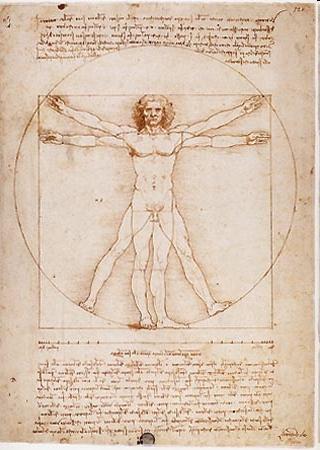
\includegraphics[width=3cm]{images/davinci.png}
\end{textblock*}
\end{frame}

\begin{frame}
\frametitle{Modern English (1700 -  \dots)}
\begin{itemize}
\item By 1700 English has (nearly) reached \\ its present form.		
\item Increasing standardization 
\item Samuel Johnson's Dictionary of the English Language.
\item Present Day English is considered to be one kind of Modern English.
\item Analytic language (Modern English = period of lost inflection)
\item Relation of words is indicated by a relatively fixed word order.
\end{itemize}
\begin{textblock*}{10cm}(8.3cm,1.3cm)
\includegraphics[width=4cm]{images/dictionary.png}
\end{textblock*}
\end{frame}

\begin{frame}
\frametitle{Modern English (1700 - \dots)}
\begin{itemize}
\item ModE's lexicon can be assigned to three different origins:
\begin{itemize}
\item Germanic words that survived since OE
\item Vocabulary adopted from Latin, French and other European tongues	
\item Words that have their origin in the geographical expansion of the British Empire
\end{itemize}
\item Pronunciation is much the same as in EmodE
\item Rise of Received Pronunciation in  the early 20^{th} century
\item Received Pronunciation is an accent that, concerning linguistics, serves  as reference in phonetics and phonology.
\item At the beginning of the 21^{st} century, the regional varieties exhibit an increase in independence and begin more and more to form their own $"$standards$"$.
\end{itemize}
\end{frame}

\begin{frame}
\frametitle{English as a Global Language}
\begin{itemize}
\item Up to 1200 English was limited to the British Isles 
\item Phases of expansion	
\begin{itemize}
\item Spreading of English across the British Isles
\item Spreading beyond the British Isles due to colonization!
\end{itemize}
\item Native language of about 340.000.000 people 
\item 2^{nd} language in about 60 countries
\item Major global language
\end{itemize}
\end{frame}

\begin{frame}
\frametitle{English as a Global Language}
\begin{itemize}
\item English today is the most widely \\ used language
\item Braj Kachru accounts for the \\ different functions English has \\ in different territories by \\ introducing the model of the three circles of English.
\begin{itemize}
\item 1st circle: English is native language
\item 2nd circle: English is second language
\item 3rd circle: English is a foreign language, but is widely understood
\end{itemize}
\end{itemize}
\begin{textblock*}{10cm}(8.3cm,1.3cm)
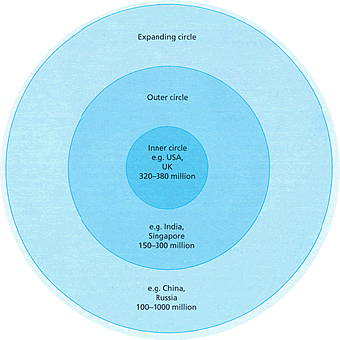
\includegraphics[width=4cm]{images/kachrucircle.png}
\end{textblock*}
\end{frame}

\begin{frame}
\frametitle{English as a Global Language}
\begin{itemize}
\item English is the first truly international language
\item Its the global lingua franca (also in intra-national communication, e.g. India)
\item Internationally and cross-culturally there are various domains where English is used as lingua franca:
\begin{itemize}
\item Economy 
\item Politics 
\item Science 
\item International travel 
\item Trade and transport 
\item Modern technology (computer and  Internet related terminology)
\end{itemize}
\end{itemize}
\end{frame}

\begin{frame}
\frametitle{The Future of English}
\begin{itemize}
\item Former third world countries in South Asia and Africa, especially grow rapidly by economic standards and in terms of population
\item The number of speakers in highly developed countries (Western culture) is by comparison in decline
\item In the future we will probably see an increase in independence of varieties which are still regarded as $"$inferior$"$ sub-varieties of English
\end{itemize}
\end{frame}

\begin{frame}
\frametitle{The Future of English}
\begin{itemize}
\item Will English be substituted by another language, e.g. Mandarin (Chinese)?
\begin{itemize}
\item Well, we don't know, but \dots
\item English is the established lingua franca and it appears to be rather unlikely that this will change anytime soon.
\item Countries were English is L2 are among those nations that gain importance (India, Philippines, Tanzania, Nigeria,\dots).
\item Pidgin and creole varieties will become more widespread and will gain prestige (accepted alternative standards)
\end{itemize}
\end{itemize}
\end{frame}

\begin{frame}
\frametitle{The Future of English}
\begin{itemize}
\item Do we need a universal language?
\begin{itemize}
\item Between 1880 and 1907 53 universal languages were proposed (thousands throughout our attested history)
\item Most universal languages are forgotten (lack of speakers)
\item Recent history has shown language policy to be a highly emotional issue, the language of a country often symbolizing its independence and nationalism. (Baugh and Cable 1991: 7) 
\end{itemize}
\end{itemize}
\end{frame}

\begin{frame}
\frametitle{Orthography and Pronunciation}
Different spellings for same sound, e.g. for \textipa{[i:]}\\
\begin{tabularx}{\textwidth}{lll}
$<$ae$>$ Caesar	& $<$eo$>$ people & $<$ey$>$ key\\
$<$ay$>$ quay & $<$ea$>$ sea, tea & $<$i$>$ ski, police,\\
$<$e$>$ be & $<$ee$>$ sneeze & $<$ie$>$ field, yield\\
$<$ei$>$ seize & $<$oe$>$ Phoenix & \\\\
\end{tabularx}
Same spelling for different sounds, e.g. $<$ea$>$\\
\begin{tabularx}{\textwidth}{ll}
\textipa{[e@]} bear & \textipa{[A:]} heart\\
\textipa{[I@]} beard & \textipa{[e]} head, dead\\
\textipa{[3:]} heard, learn & \textipa{[i:]} heat, meat\\\\
\end{tabularx}
Silent or missing letters: know, honest, debt \textipa{[j]} in use, fuse.\\
\end{frame}

%%%%%%%%%%%%%%%%%%%%%%%%%%%%%%%%%%%%%%%%%%%%%%%%%%
%%% Phonetics: Phones and Phonemes

\section{Phonetics}
\begin{frame}
\frametitle{Phonetics}
Phonetics tries to determine and describe the properties of sounds used in communication.\\
Articulatory Phonetics
\begin{itemize}
\item How are speech sounds produced?
\end{itemize}
Acoustic Phonetics
\begin{itemize}
\item How do speech sounds "travel" from one \\
person to another?\\
\end{itemize}
Auditory Phonetics 
\begin{itemize}
\item How do speaker and hearer perceive\\
these sounds?
\end{itemize}
\begin{textblock*}{4cm}(9cm,3.5cm)
\includegraphics[width=2cm]{images/vocaltract.jpg}
\end{textblock*}
\begin{textblock*}{6cm}(9cm,5.5cm)
\includegraphics[width=2cm]{images/soundwaves.jpg}
\end{textblock*}
\begin{textblock*}{8cm}(9cm,7.5cm)
\includegraphics[width=2cm]{images/auditorysystem.png}
\end{textblock*}
\end{frame}

\begin{frame}
\frametitle{Articulatory Phonetics}
\begin{itemize}
\item Describes sounds with regard\\
to the organs of speech
\item Which organs of speech are\\
involved?
\item How are these organs\\
manipulated?
\end{itemize}
\begin{textblock*}{8cm}(7cm,2.5cm)
\includegraphics[width=5cm]{images/organsofspeech.png}
\end{textblock*}
\end{frame}

\begin{frame}
\frametitle{Acoustic Phonetics}
\begin{itemize}
\item What happens to the air\\
between speaker and listener? 
\item Study of the acoustic\\
properties of speech sounds
\item Use of  technical devices\\
(e.g. sonograph) to analyze the\\
frequencies that sounds consist of.
\end{itemize}
\begin{textblock*}{8cm}(7cm,2.5cm)
\includegraphics[width=5cm]{images/spectrogram.png}
\end{textblock*}
\end{frame}

\begin{frame}
\frametitle{Auditory Phonetics}
\begin{itemize}
\item How are speech sounds perceived\\
by (the ear of) the speaker and the listener?  
\item How does the brain distinguish between sounds?
\item How much do we "need to understand"?
\end{itemize}
\begin{textblock*}{8cm}(8cm,1.5cm)
\includegraphics[width=4cm]{images/ear.png}
\end{textblock*}
\begin{textblock*}{8cm}(7cm,6.5cm)
\includegraphics[width=5cm]{images/brainimaging.png}
\end{textblock*}
\end{frame}

\begin{frame}
\frametitle{Auditory Phonetics}
\begin{itemize}
\item How are speech sounds perceived\\
by (the ear of) the speaker and the listener?  
\item How does the brain distinguish between sounds?
\item How much do we "need to understand"?
\end{itemize}
\begin{textblock*}{8cm}(8cm,1.5cm)
\includegraphics[width=4cm]{images/ear.png}
\end{textblock*}
\begin{textblock*}{8cm}(7cm,6.5cm)
\includegraphics[width=5cm]{images/brainimaging.png}
\end{textblock*}
\end{frame}

\begin{frame}
\frametitle{Speech Sound Production System}
\begin{tabularx}{\textwidth}{Y YY}
Lungs & Larynx (voice box) & Vocal tract\\[5cm]
\end{tabularx}
\begin{textblock*}{.2cm}(.2cm,4cm)
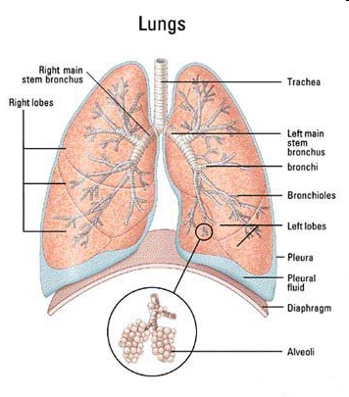
\includegraphics[width=4cm]{images/lungs.png}
\end{textblock*}
\begin{textblock*}{4cm}(4cm,4cm)
\includegraphics[width=4cm]{images/voicebox.png}
\end{textblock*}
\begin{textblock*}{6cm}(7cm,3.5cm)
\includegraphics[width=5cm]{images/vocaltract.jpg}
\end{textblock*}
\end{frame}

\begin{frame}
\frametitle{Egressive Pulmonic Airstream Mechanism}
\begin{itemize}
\item Mechanism that produces an air stream that is pushed up from the lungs and leaves the body through the mouth or nose.
\item Produces almost all speech sounds in English with the exception of sounds which we produce when we are in emotional distress (e.g. fear) or when we are counting to ourselves.
\end{itemize}
\end{frame}

\begin{frame}
\frametitle{Organs of Speech}
\begin{itemize}
\item The primary function of the\\
organs of speech is/was in fact\\
not speech itself, because the\\
speech organs evolved primarily\\
for \dots
\begin{itemize}
\item chewing, biting,\\
(especially teeth) 
\item sucking, mouth hygiene\\
(tongue)
\item to prevent us from choking\\
on something (soft palate) 
\item to enable us to strain\\
(hold the breath) when we want to lift something heavy.
\end{itemize}
\end{itemize}
\begin{textblock*}{4cm}(7.5cm,3cm)
\includegraphics[width=5cm]{images/mouth.png}
\end{textblock*}
\end{frame}

\begin{frame}
\frametitle{Organs of Speech}
\begin{itemize}
\item alveolar ridge (Zahndamm)
\item hard palate (harter Gaumen)
\item velum/soft palate\\(weicher Gaumen/ Gaumensegel)
\item uvula (Z{\"a}pfchen)
\item pharynx (Rachen)
\item epiglottis (Stimmritze)
\item larynx (Kehlkopf)
\item vocal cords/folds (Stimmb{\"a}nder)
\item trachea (Luftr{\"o}hre)
\end{itemize}
\begin{textblock*}{4cm}(7.5cm,3cm)
\includegraphics[width=5cm]{images/mouth.png}
\end{textblock*}
\end{frame}

\begin{frame}
\frametitle{Sound Categorization}
\begin{tabularx}{\textwidth}{Y YY}
Vowels & Approximants & Consonants\\
& Laterals &\\
& Semivowels &\\
\end{tabularx}
\begin{textblock*}{2cm}(2cm,2.5cm)
\includegraphics[width=1.5cm]{images/vowelsmouth.png}
\end{textblock*}
\begin{textblock*}{4cm}(1cm,5cm)
\includegraphics[width=4cm]{images/vowelchart.png}
\end{textblock*}
\begin{textblock*}{2cm}(9cm,2.5cm)
\includegraphics[width=1.5cm]{images/consonantsmouth.png}
\end{textblock*}
\begin{textblock*}{6cm}(7.5cm,6cm)
\includegraphics[width=5cm]{images/consonantschart.png}
\end{textblock*}
\begin{textblock*}{6cm}(7.5cm,7.3cm)
\includegraphics[width=5cm]{images/lateralschart.png}
\end{textblock*}
\end{frame}

\begin{frame}
\frametitle{Vowels}
\begin{tabularx}{\textwidth}{YYYY}
\textipa{I} & p\uline{i}t & \textipa{O:} & b\uline{o}rn \\
\textipa{e} & p\uline{e}t & \textipa{u:} & b\uline{oo}n \\
\textipa{\ae} & p\uline{a}t & \textipa{aI} & b\uline{i}te \\
\textipa{6} & p\uline{o}t & \textipa{eI} & b\uline{ai}t \\
\textipa{2} & b\uline{u}t & \textipa{OI} & b\uline{o}y \\
\textipa{U} & b\uline{oo}k & \textipa{@U} & t\uline{oe} \\
\textipa{@} & moth\uline{er} & \textipa{aU} & h\uline{ou}se \\
\textipa{i:} & b\uline{ea}n & \textipa{U@} & p\uline{oo}r \\
\textipa{3:} & b\uline{u}rn & \textipa{I@} & \uline{ea}r \\
\textipa{A:} & b\uline{a}rn & \textipa{e@} & \uline{ai}r \\
\end{tabularx}
\end{frame}

\begin{frame}
\frametitle{Vowels}
\begin{textblock*}{4cm}(3.5cm,2cm)
\includegraphics[width=5cm]{images/vowelchartempty.png}
\end{textblock*}
\end{frame}

\begin{frame}
\frametitle{Vowels}
\begin{itemize}
\item Produced by \dots
\begin{itemize}
\item opening the lips 
\item vibrating the vocal cords 
\item raising the tongue to\\
various heights. 
\end{itemize}
\item Vowel sounds are produced\\
without obstruction of the air\\
stream.
\item Can form the nucleus of syllables\\
(central, pulse-bearing part of syllables).
\item Vowels are generally more sonorous than consonants.
\item In English, vowel sounds are always voiced.
\end{itemize}
\begin{textblock*}{3cm}(7.5cm,2cm)
\includegraphics[width=5cm]{images/vowelchart.png}
\end{textblock*}
\end{frame}

\begin{frame}
\frametitle{Vowels}
Categorization of vowels:
\begin{itemize}
\item Height of the tongue:
\begin{itemize}
\item high (sometimes also closed)
\item mid (sometimes also mid-closed/mid-open)
\item low (sometimes also open)
\end{itemize}
\item Position of highest part of tongue:
\begin{itemize}
\item front
\item central
\item back
\end{itemize}
\item State of lips:
\begin{itemize}
\item Rounded or unrounded (latter sometimes spread and neutral)
\item Roundedness: only affects \textipa{U, O:}, and \textipa{u:} in English.
\end{itemize}
\end{itemize}
\end{frame}

\begin{frame}
\movie[width=8cm]{\includegraphics[width=7cm]{images/tonguemovement.png}}{movies/voweltongue.avi}
\end{frame}

\begin{frame}
\frametitle{Consonants}
\begin{itemize}
\item Produced with obstruction of the air-stream, e.g. lip against lip \textipa{[m]}, tongue between teeth \textipa{[D]}, tongue against teeth-ridge \textipa{[t]} and \textipa{[d]}, tongue against soft-palate \textipa{[g]}, etc.
\end{itemize}
\begin{textblock*}{3cm}(3cm,6cm)
\includegraphics[width=8cm]{images/consonantchart.png}
\end{textblock*}
\end{frame}

\begin{frame}
\frametitle{Consonants}
\begin{tabularx}{\textwidth}{YYYY}
\textipa{p} & \uline{p}ip & \textipa{Z} & mea\uline{s}ure \\
\textipa{b} & \uline{b}ib & \textipa{h} & \uline{h}en \\
\textipa{t} & \uline{t}en & \textipa{tS} & \uline{ch}urch \\
\textipa{d} & \uline{d}en & \textipa{dZ} & ju\uline{dg}e \\
\textipa{k} & \uline{c}at & \textipa{m} & \uline{m}an \\
\textipa{g} & \uline{g}et & \textipa{n} & \uline{n}ow \\
\textipa{f} & \uline{f}ish & \textipa{N} & si\uline{ng} \\
\textipa{T} & \uline{th}igh & \textipa{l} & \uline{l}et \\
\textipa{D} & \uline{th}is & \textipa{r} & \uline{r}ide \\
\textipa{s} & \uline{s}et & \textipa{w} & \uline{w}et \\
\textipa{z} & \uline{z}oo & \textipa{j} & \uline{y}et \\
\textipa{S} & \uline{s}hip & \textipa{v} & \uline{v}ery \\
\end{tabularx}
\end{frame}

\begin{frame}
\frametitle{Consonant classification}
\begin{itemize}
\item Consonants are classified according to their voicedness and according to where and how the air stream is obstructed. The relevant criteria, hence, are... 
\item State of glottis
\begin{itemize}
\item voicedness or voicelessness (voicing)
\end{itemize}
\item Place of articulation
\begin{itemize}
\item bilabial, labio-dental, alveolar, glottal, etc.
\end{itemize}
\item Manner of articulation
\begin{itemize}
\item plosive, nasal, etc.
\end{itemize}
\end{itemize}
\end{frame}

\begin{frame}
\frametitle{Consonant classification}
\begin{itemize}
\item Soft palate/velum (velar)\\
\textipa{k, g, N} 
\item Hart palate (palatal)\\
\textipa{j}
\item Palate/alveolar (palatal-alveolar)\\
\textipa{S, Z, tS, DZ} 
\item Alveolar ridge (alveolar)\\
\textipa{t, d, n, s, z, l, \*r}
\item Teeth (dental)\\
\textipa{T, D}
\item Lips (labial)\\
\textipa{p, b, m, w} (bilabial); \textipa{f, v} (labio-dental)
\end{itemize}
\begin{textblock*}{3cm}(8cm,2cm)
\includegraphics[width=4cm]{images/soundsorgans.png}
\end{textblock*}
\end{frame}

\begin{frame}
\frametitle{Consonant classification}
\begin{itemize}
\item Plosives (also called stops, Verschlusslaut)\\
\textipa{p, b, t, d, k, g}
\item Fricatives ("with friction", Reibelaut)\\
\textipa{f, D, T, s, z, S, Z}
\item Affricates (plosives and homorganic fricatives, Affrikate)\\
\textipa{tS, dZ}\\
(compare German: ts, pf, ?ps)
\item Nasals ("through the nose", Nasale)\\
\textipa{m, n, N}
\item Approximants ("getting close", N{\"a}herungslaut)\\
\textipa{w, \*r, l, j}
\end{itemize}
\end{frame}

\begin{frame}
\frametitle{Transcription}
\Tree [.Transcription [.Phonetic [.narrow ring:\textipa{[{\*r}\~IN]} till:\textipa{[t\super h\~I\textbeltl]} ] [.broad ring:\textipa{[\*rIN]} till:\textipa{[tI\textbeltl]} ] ][.Phonemtic ring:\textipa{/rIN/} till:\textipa{/tIl/} ] ]\\
\hfill \footnotesize{\citep[adapted from][61]{kortmann2001linguistik}}\\
\end{frame}

%%%%%%%%%%%%%%%%%%%%%%%%%%%%%%%%%%%%%%%%%%%%%%%%%%
%%% Phonology: Allophony and Syllables
\section{Phonology}
\begin{frame}
\frametitle{Phonology: Today's topics and terms}
\begin{itemize}
\item Segmental and suprasegmental phonology
\item Phoneme
\item Minimal Pair
\item Allophone
\item Free variation and complementary distribution
\item Syllable
\item Phonological processes
\item Word stress and sentence stress
\end{itemize}
\end{frame}

\begin{frame}
\frametitle{Phonology: Allophony and Syllables}
\footnotesize{\Tree [.\textipa{/k/} [.\textipa{/k/} [.\textipa{[k]}_{1} ] [.\textipa{[k]}_{2} ] [.\textipa{[k]}_{3} ] [.\textipa{...} ] [.\textipa{[k]}_{n} ] ] [.\textipa{/k\super h/} [.\textipa{[k\super h]}_{1} ] [.\textipa{[k\super h]}_{2} ] [.\textipa{[k\super h]}_{3} ] [.\textipa{...} ] [.\textipa{[k\super h]}_{n} ] ] ] }
\begin{textblock*}{6cm}(6.4cm,3.65cm)
\textit{Phoneme (abstract category)}
\end{textblock*}
\begin{textblock*}{5cm}(9.2cm,5.15cm)
\textit{Allophones (abstract variants/subcategories)}
\end{textblock*}
\begin{textblock*}{6cm}(3.8cm,7cm)
\textit{Phones (concrete realizations)}
\end{textblock*}
\begin{textblock*}{6cm}(1cm,3cm)
Functional level (Phonology)
\end{textblock*}
\begin{textblock*}{6cm}(1cm,8cm)
Descriptive level (Phonetics)
\end{textblock*}
\end{frame}

\begin{frame}
\frametitle{Phonology}
\begin{itemize}
\item Concerned with the speakers knowledge of the sound system of languages.
\item Studies the so-called sound inventory, its function and (mental) organization.
\item Study of sounds on the functional level.
\end{itemize}
\footnotesize{\Tree [.Phonology [.{Segmental phonology} {examines the function of \\ individual segments (phonemes/phones)} ] [.{Suprasegmental phonology} {concerned with features \\ of speech that extend \\ over more than one segment \\ (rhyme, intonation, etc.)} ] ] }
\end{frame}

\begin{frame}
\begin{textblock*}{8.5cm}(2cm,4cm)
Phonology is NOT (so much) concerned with the actual articulation of sounds! It is concerned with the function and interaction of phonemes!
\end{textblock*}
\end{frame}

\begin{frame}
\frametitle{Segmental Phonology}
\begin{itemize}
\item Concerned with the function of segments.
\item Some segments distinguish meaning:\\
\begin{exe}
\ex \textipa{/\uline{l}ait/} : \textipa{/\uline{b}ait/} 
\end{exe}
\item If two sounds differ/are in contrast/are distinctive/are in opposition, the contrasting units are called \textit{phonemes}.
\end{itemize}
\end{frame}

\begin{frame}
\frametitle{Phonemes}
\begin{itemize}
\item Phonemes are the smallest meaning-distinguishing units in language.
\item Phonemes are not actual sounds (they are not themselves articulated) but abstract mental representations (ideal sounds) that underlie concrete articulation. 
\item Phonemes are identified by applying a \textit{minimal pair test}. 
\item The so-called phoneme inventory of a given language encompasses all contrasting sounds that are identified by the minimal pair test.
\end{itemize}
\end{frame}

\begin{frame}
\frametitle{Minimal pair test}
\begin{itemize}
\item Chose words that \dots 
\begin{itemize}
\item have the same number of segments
\item differ in only one sound (segment) 
\item differ in meaning
\end{itemize}
\item \textipa{/s/} and \textipa{/f/} are phonemes in English because they create a difference in meaning.
\end{itemize}
\begin{textblock*}{5cm}(8.5cm,3.5cm)
\begin{tabularx}{3.5cm}{l|ccc}
\hline
& \multicolumn{3}{c}{Segment} \\
Word & 1 & 2 & 3\\
\hline
sun & \textipa{s} & \textipa{2} & \textipa{n}\\
fun & \textipa{f} & \textipa{2} & \textipa{n}\\
\hline
\end{tabularx}
\end{textblock*}
\end{frame}

\begin{frame}
\begin{textblock*}{8.5cm}(2cm,2cm)
Every language uses a relatively small number of sounds which are combined in a relatively large number of different ways. [\dots] The enormous numbers of different sounds that can be found in any given language can be classified and grouped into a small number of basic sounds.\\ \hfill{(Nathan 2008: 28)}
\end{textblock*}
\begin{textblock*}{8.5cm}(1cm,5.5cm)
\footnotesize{\Tree [.Sounds [.{(Allo-)phones} {enormous number of different sounds} ] [.{Phonemes} {small number of basic sounds} ] ] }
\end{textblock*}
\end{frame}

\begin{frame}
\frametitle{Allophones}
\begin{itemize}
\item Allo ~$"$other$"$_{Greek} + phone ~$"$sound$"$_{Greek}
\item Subcategories of phonemes (basic $"$sounds$"$).
\item Allophonic variation occurs in all languages, but the patterning of phonemes and allophones is language specific.
\begin{itemize}
\item Laymen regard allophones of one phoneme as the same sound. 
\item Phonetically (slightly) different. 
\end{itemize}
\end{itemize}
\end{frame}

\begin{frame}
\frametitle{Allophones}
\begin{textblock*}{8.5cm}(1cm,2.5cm)
\footnotesize{\Tree [.Allophones [.{Allophones in free variation \\ (Free Variants)} {can occur in the \\ same environment} ] [.{Allophones in \\ complementary distribution} {cannot occur in the \\ same environment
} ] ] }
\end{textblock*}
\begin{textblock*}{5cm}(1.5cm,6.4cm)
\begin{tabularx}{3.5cm}{l|ccc}
\hline
& \multicolumn{3}{c}{Segment} \\
Word & 1 & 2 & 3\\
\hline
rip & \textipa{\*r} & \textipa{I} & \textipa{p}\\
rip & \textipa{\*r} & \textipa{I} & \textipa{\r*p}\\
rip & \textipa{\*r} & \textipa{I} & \textipa{Pp}\\
\hline
\end{tabularx}
\end{textblock*}
\begin{textblock*}{5cm}(6.5cm,6.4cm)
\begin{tabularx}{3.5cm}{l|ccc}
\hline
& \multicolumn{3}{c}{Segment} \\
Word & 1 & 2 & 3\\
\hline
til & \textipa{t} & \textipa{I} & \textipa{\textbeltl}\\
love & \textipa{l} & \textipa{2} & \textipa{v}\\
lol & \textipa{l} & \textipa{6} & \textipa{\textbeltl}\\
\end{tabularx}
\end{textblock*}
\end{frame}

\begin{frame}
\frametitle{Allophones in complementary distribution}
\begin{textblock*}{10cm}(1cm,2.5cm)
\begin{itemize}
\item Allophones in complementary distribution are variants of the same phoneme that cannot occur in the same phonetic or phonological environment. 
\item Allophones in complementary distribution are like \dots
\end{itemize}
\end{textblock*}
\begin{textblock*}{8.5cm}(2cm,5.3cm)
\footnotesize{\Tree [.{Cannot occur in the same environment!} [.{Louis Lane is in danger} ] [.{Daily Planet office} ] ] }
\end{textblock*}
\begin{textblock*}{8cm}(.3cm,5.5cm)
\includegraphics[width=2cm]{images/superman.png}
\end{textblock*}
\begin{textblock*}{8cm}(10cm,5.5cm)
\includegraphics[width=2cm]{images/clarkkent.jpg}
\end{textblock*}
\end{frame}

\begin{frame}
\frametitle{Allophones in complementary distribution}
\begin{textblock*}{10cm}(1cm,2.5cm)
\begin{itemize}
\item Clear \textipa{l} and dark \textipa{\textbeltl} are allophones in complementary distribution.
\end{itemize}
\end{textblock*}
\begin{textblock*}{8.5cm}(2.1cm,4cm)
\footnotesize{\Tree [.{ Phoneme \textipa{/l/}} [.{Clear \textipa{[l]} \\ as in $<$lip$>$ occurs \\ before vowels} ] [.{Dark \textipa{[\textbeltl]} \\ as in $<$feel$>$ occurs before \\ consonants and silences} ] ] }
\end{textblock*}
\begin{textblock*}{8cm}(.3cm,5.5cm)
\includegraphics[width=2cm]{images/clearl.png}
\end{textblock*}
\begin{textblock*}{8cm}(10cm,5.5cm)
\includegraphics[width=2cm]{images/darkl.png}
\end{textblock*}
\end{frame}

\begin{frame}
\frametitle{Phonotactic Rules}
\begin{itemize}
\item Rules that define the translation of  knowledge about language into actual speech sounds.
\item Such rules are not universal, but language specific.
\item In English, the voiced alveolar lateral approximant becomes velarised when it occurs before a consonant or silence:
\begin{itemize}
\item phonetic form \textipa{[l2\textbeltl]} and \textipa{[bI\textbeltl d]} 
\item phonemic form \textipa{/l2l/} and \textipa{/bIld/}
\end{itemize}
\item In German, all word final plosives become devoiced. Thus $-$ in terms of voicing $-$ there is no difference between the pronunciation of $<$Rad$>$ and $<$Rat$>$.
\end{itemize}
\end{frame}

\begin{frame}
\frametitle{Distinctive Features}
\begin{itemize}
\item Distinctive feature of minimal pairs \textipa{[zi:\textbeltl]} and \textipa{[si:\textbeltl]} or \textipa{[bIt]} and \textipa{[bId]} is voicing (manner and place of articulation are identical).
Sounds can be characterised by bundles of distinctive features marked by (-) or (+).\\[.5cm]
\begin{tabularx}{6.5cm}{l|cccc}
& \multicolumn{4}{c}{Sound}\\
Feature& \textipa{/b/} & \textipa{/d/} & \textipa{/g/} & \textipa{/k/}\\
\hline
plosive & + & + & + & + \\
voiced & + & + & + & - \\
(bi-)labial & + & - & - & - \\
alveolar & - & + & - & - \\
velar & - & - & + & + \\
\hline
\end{tabularx}
\end{itemize}
\end{frame}

\begin{frame}
\frametitle{Suprasegmental Phonology}
\begin{itemize}
\item Suprasegmental phonology deals with phonological properties that extend over more than a single segment.
\end{itemize}
\footnotesize{\Tree [.{Suprasegmental Phonology} [.{deals with the \\ combination of segments into \\ larger units (syllables) } ] [.{studies properties of \\ larger stretches of speech \\ (prosody, intonation, stress, ...) } ] ] }
\end{frame}

\begin{frame}
\frametitle{Syllable}
\begin{itemize}
\item Phonological units above phoneme level
\item Smallest rhythmic unit of speech
\item Monosyllabic words: words with only one syllable
\item Polysyllabic words: words with at least two syllables.
\item In English, all syllables contain a nucleus (or peak, core, center), a coda and an onset.\\
\footnotesize{\Tree [.Syllable [.Onset [.C \textipa{[l]} ] ] [.Rhyme [.Nucleus [.V \textipa{[ai]} ] ] [.Coda [.C \textipa{[k]} ] ] ] ] }
\end{itemize}
\end{frame}

\begin{frame}
\frametitle{Syllable}
\begin{itemize}
\item Nucleus
\begin{itemize}
\item central element of a syllable.
\item usually a vowel sound (V).
\end{itemize}
\item Coda
\begin{itemize}
\item up to 4 consonants that follow the vowel (CCCC).
\end{itemize}
\item Onset
\begin{itemize}
\item up to 3 consonants that precede the vowel (CCC).
\end{itemize}
\item Rhyme
\begin{itemize}
\item nucleus and coda form the \textit{rhyme}
\end{itemize}
\item Open Syllables are syllables in which the coda is empty.
\item Closed Syllables are syllables in which one or more consonants follow the nucleus.
\end{itemize}
\end{frame}

\begin{frame}
\frametitle{Phonological processes}
\begin{itemize}
\item Sounds are changed to fit their surrounding/ environment and speakers adjust the sounds they produce according to rules of their language without realizing it.
\item Such adaptations are known since the 19th century and called $"$divergences$"$.
\item Divergences are either \dots
\begin{itemize}
\item physiophonetic: phonetically motivated
\item paleophonetic: conventionally or historically motivated
\end{itemize} 
\end{itemize}
\end{frame}

\begin{frame}
\frametitle{Phonological processes}
\begin{textblock*}{6.5cm}(7cm,3cm)
\begin{tabularx}{5cm}{ll}
Word/phrase & Transcription\\
\hline
dogs & \textipa{[d6g z]}\\
cats & \textipa{[k\ae t s]}\\
faxes & \textipa{[f\ae ks Iz]}\\
\hline
he goes & \textipa{[hIgoU z]}\\
he walks & \textipa{[hIwO:k s]}\\
\hline
Rick's & \textipa{[rIk s]}\\
John's & \textipa{[dZ6n z]}\\
\hline
Church Street & \textipa{[tS3tSt{\*r}i:t]}\\
\hline
\end{tabularx}
\end{textblock*}
\begin{textblock*}{6cm}(1cm,2.5cm)
\begin{itemize}
\item Progressive Assimilation
\begin{itemize}
\item The noun plural marker, the singular present tense (3rd person) marker, the possessive marker, and sibilants  always agree in voicing with the proceeding sound.
\item Progressive assimilation moves forward to the following segment.
\end{itemize}
\end{itemize}
\end{textblock*}
\end{frame}

\begin{frame}
\frametitle{Phonological processes}
\begin{textblock*}{6.5cm}(7cm,2.8cm)
\begin{tabularx}{5cm}{ll}
Word/phrase & Transcription\\
\hline
ten bats & \textipa{[temb\ae ts]}\\
don't be & \textipa{[d@UmpI]}\\
\hline
\end{tabularx}
\end{textblock*}
\begin{textblock*}{10.5cm}(1cm,2.5cm)
\begin{itemize}
\item Regressive Assimilation
\begin{itemize}
\item All nasals become \textipa{[m]} \\ before \textipa{/p/}, \textipa{/b/}, and \textipa{/m/}.
\item All nasals become \textipa{[N]} \\ before \textipa{/k/} or \textipa{/g/}.
\item Regressive assimilation moves backwards to the preceding segment.
\end{itemize}
\item Reciprocal Assimilation
\begin{itemize}
\item Reciprocal Assimilation \\ occurs if two neighbouring \\ sounds are combined to \\ form a new sound.
\end{itemize}
\end{itemize}
\end{textblock*}
\begin{textblock*}{6.5cm}(7cm,6.5cm)
\begin{tabularx}{5cm}{ll}
Word/phrase & Transcription\\
\hline
don't you & \textipa{[d@UntSu:]}\\
kiss you & \textipa{[kISu:]}\\
\hline
\end{tabularx}
\end{textblock*}
\end{frame}

\begin{frame}
\frametitle{Phonological processes}
\begin{itemize}
\item Assimilation
\begin{itemize}
\item Assimilating effect or influence on sounds by neighboring sounds.
\item Most frequent type of assimilation is regressive assimilation.
\item Tendency to produce homorganic sounds, 
assimilation with respect to place of articulation to increase ease of articulation
\end{itemize}
\item Linguistic economy
\begin{itemize}
\item The $"$principle of minimal effort$"$ is mainly responsible for allophonic variation.
\end{itemize}
\end{itemize}
\end{frame}

\begin{frame}
\frametitle{Phonological processes}
\begin{textblock*}{8.5cm}(2cm,6cm)
\begin{tabularx}{8cm}{lll}
Word/phrase & Full & Reduced \\
\hline
every & \textipa{[ev@rI]} & \textipa{[evrI]} \\
family & \textipa{[f{\ae}m@lI]} & \textipa{[f{\ae}mlI]} \\
lastly & \textipa{[lA:stlI]} & \textipa{[lA:slI]} \\
left behind & \textipa{[lefbIhaInd]} & \textipa{[leftbIhaInd]}\\
\hline
\end{tabularx}
\end{textblock*}
\begin{textblock*}{10.5cm}(1cm,2.5cm)
\begin{itemize}
\item Deletion
\begin{itemize} 
\item Deletion refers to cases in which sounds are omitted.
\item Syncope
\begin{itemize}
\item deletion in the middle of a word.
\end{itemize}
\item Apocope
\begin{itemize}
\item deletion at the end of a word.
\end{itemize}
\end{itemize}
\end{itemize}
\end{textblock*}
\end{frame}

\begin{frame}
\frametitle{Phonological processes}
\begin{itemize}
\item Insertion
\begin{itemize}
\item Prothesis 
\begin{itemize}
\item Sound is added at the beginning of a word
\item Spanish does not permit \textipa{/sk/} clusters at the beginning of words.
\item School (sp.) $<$escuela$>$ = \textipa{[eskwel2]}	
\end{itemize}
\item Epenthesis 
\begin{itemize}
\item Sound is inserted in the middle of a word or phrase.
\item athlete = \textipa{[\ae T@li:t]}
\end{itemize}
\end{itemize}
\end{itemize}
\end{frame}

\begin{frame}
\frametitle{Phonological processes}
\begin{itemize}
\item Insertion
\begin{itemize}
\item Excrescence
\begin{itemize}
\item sound added is a consonant.
\end{itemize}
\item Anaptyxis
\begin{itemize}
\item sound added is a vowel (schwa, i.e. \textipa{/@/})
\end{itemize}
\item Liaison
\begin{itemize}
\item Linking r in non-rhotic dialects (if following word begins with a vowel)
\item $<$My car is gone$>$ = \textipa{[maIkA:^{r}Isg6n]}
\end{itemize}
\item Intrusion
\begin{itemize}
\item Intrusive r between words, even if there is no $<$r$>$ in the spelling.
\item $<$law and order$>$ = \textipa{[lO:^{r}@nO:d@]}
\end{itemize}
\end{itemize}
\end{itemize}
\end{frame}

\begin{frame}
\frametitle{Stress}
\begin{itemize}
\item \dots contributes to understanding.
\item \dots force used to produce a syllable.	
\item \dots indicated by \textipa{cvc"cvc}.
\item \dots in longer polysyllabic words, we can distinguish between primary stress \textipa{cvc"cvc} and secondary stress \myipa{""cvcv"cvcv}.
\item \dots important feature in structure not only of words, but also of phrases and sentences.
\footnotesize{
\begin{exe}
\ex \begin{xlist}
\ex \textipa{[im"p6^{r}t]} (import; verb) 
\ex \myipa{["imp6^{r}t]} (import; noun)
\end{xlist}
\end{exe}
\begin{exe}
\ex \begin{xlist}
\ex \textipa{[en"trA:ns]} (entrance; verb meaning delight, enchant)
\ex \myipa{["entr@ns]} (entrance; noun meaning door, gate)
\end{xlist}
\end{exe}}
\end{itemize}
\end{frame}

\begin{frame}
\frametitle{Stress}
\begin{itemize}
\item Word stress
\begin{itemize}
\item English words with two syllables or more will have some syllable more prominent that others.
\item Due to the massive influx of foreign vocabulary, word stress is generally not predictable (rule of thumb for word stress: always stress the last but one syllable)
\item Word stress can be meaning distinguishing.
\footnotesize{
\begin{exe}
\ex \begin{xlist}
\ex \textipa{[im"p6^{r}t]} (import; verb) 
\ex \myipa{["imp6^{r}t]} (import; noun)
\end{xlist}
\end{exe}}
\item Word stress can cause vowel change and languages vary concerning whether their vowels are weakened when they appear in unstressed syllables (as in English, Russian) or not (as in German).
\end{itemize}
\end{itemize}
\end{frame}

\begin{frame}
\frametitle{Stress}
\begin{itemize}
\item Sentence stress
\begin{itemize}
\item Sentence stress depends to a larger part on rhythm. 
\item Rhythm refers to the distribution of stressed syllables in a phrase or sentence.
\item Lexical items that carry main semantic content (nouns, adjectives, verbs, adverbs) take stress. 
\item Monosyllabic function words (grammatical PoS like prepositions, conjunctions personal pronouns) do no take stress and their vowels become schwas.	
\end{itemize}
\end{itemize}
\end{frame}

\begin{frame}
\frametitle{Stress}
\begin{itemize}
\item Shift Stress (Switch stress)
\begin{itemize}
\item Shift stress refers to \\ 
situations in which \\ 
syllables with primary \\ 
stress in citation \\ 
form become unstressed.
\item Shift stress affects \\ 
words (Adj) with more\\ 
than one stress in \\ 
larger constructions, \\ 
e.g. in NPs.
\item Shift stress is typically \\ 
English.
\item It involves word and sentence stress.
\end{itemize}
\end{itemize}
\begin{textblock*}{3cm}(7cm,2cm)
\includegraphics[width=5cm]{images/shiftstress.png}
\end{textblock*}
\end{frame}

\begin{frame}
\frametitle{Stress}
\begin{itemize}
\item Contrastive Stress (Emphatic Stress)
\begin{itemize}
\item Usually the last stressed word is most important to the speaker.
\item If two elements within a sentence are contrasted, these elements are stressed
\begin{exe}
\ex I didn't want a \uline{small} piece of cake, I wanted a \uline{large} piece.
\end{exe}
\item Sometimes marked by making the stress extra loud.
\item Usually marked with a falling pitch, i.e. by starting the contrastive stress with higher pitch that is followed by syllables with considerably lower pitch.
\end{itemize}
\end{itemize}
\end{frame}

\begin{frame}
\frametitle{Pitch}
\begin{textblock*}{10.5cm}(1cm,2.5cm)
\begin{itemize}
\item The faster the vocal cords vibrate, the higher the pitch.
\item All voiced sounds can be produced with different pitches.
\item Pitch is usually described in terms of high and low
rises and falls in pitch across a stretch of speech
\item In English, intonation helps marking syntactic units and vaguely corresponds to punctuation.
\end{itemize}
\end{textblock*}
\end{frame}

\begin{frame}
\frametitle{Pitch}
\begin{itemize}
\item In many languages (not English) the meaning of words can differ according to pitch (such languages are called "tone languages").
\end{itemize}
\includegraphics[width=11cm]{images/tonelanguages.png}\\
\hfill \footnotesize{World Atlas of Language Structures Online}\\
\end{frame}

%%%%%%%%%%%%%%%%%%%%%%%%%%%%%%%%%%%%%%%%%%%%%%%%%%
%%% Morphology: Building Meaningful Blocks
\section{Morphology}
\begin{frame}
\frametitle{Morphology: Building Meaningful Blocks}
\begin{itemize}
\item An investigation into what elements an utterance consists of is called an morphological analysis.
\item In fact, morphology means $"$study of forms$"$ and was adopted from biology.
\item In the middle of the 19^{th} century the term was employed to describe the study of basic meaningful elements.
\item However, we do not need to look at e.g. Swahili to discover that words are made up of a number of $"$meaning bearing elements$"$ \dots\\
\dots but anyways, let's do that \dots
\end{itemize}
\end{frame}

\begin{frame}
\frametitle{Morphology: Building Meaningful Blocks}
\begin{tabularx}{\linewidth}{ccc}
Nitakupenda. & _{means} & I will love you.
\end{tabularx}
\begin{itemize}
\item How many $"$words$"$ does $"$I will love you!$"$ contain and how many words does $"$nitakupenda$"$ contain?
\item English $"$words$"$ and Swahili $"$words$"$ are not the same but maybe both contain similar $"$meaning elements$"$.
\item Maybe it is better to look at these meaning elements than at words \dots
\item But what are these elements?
\end{itemize}
\end{frame}

\begin{frame}
\frametitle{Morphology: Building Meaningful Blocks}
\begin{itemize}
\item Smallest meaning-bearing units of language. 
\item Word contains at least one morpheme
\end{itemize}
\footnotesize{\Tree[.Morphemes [.{Free morphemes} {Morphemes that are identical \\ to words (\{book\}, \{student\})
} ] [.{Bound morphemes} {Morphemes that cannot \\ stand on their own \\ (\{un\#\}, \{\#ing\}, \{\#s\}) } ] ] }
\end{frame}

\begin{frame}
\frametitle{Morphology: Building Meaningful Blocks}
\begin{tabularx}{\textwidth}{cccc}
talks & talker & talking & talked\\
\end{tabularx}
\begin{itemize}
\item All words above have one element in common (talk), but in all of the words some element is added (\{\#s\}, \{\#er\}, \{\#ing\}, \{\#ed\}).
\item Let's look at another example \dots
\end{itemize}
\begin{exe}
\ex How many morphemes is $<$\textit{tourists}$>$ made up of?
\end{exe}
\begin{tabularx}{\textwidth}{lccc}
morpheme & \{tour\#\} & \{\#ist\} & \{\#s\}\\
type & free & bound & bound\\
meaning & sth. to do with $"$tour$"$ & person doing sth. & plural\\
\end{tabularx}
\end{frame}

\begin{frame}
\frametitle{Morphology: Building Meaningful Blocks}
\footnotesize{\Tree[.Morphemes [.Free [.Lexical {\{child\}, \{teach\} } ] [.Functional { \{is\}, \{of\} } ] ] [.Bound [.Derivational {\{re\#\}, \{\#ness\} } ] [.Inflectional { \{\#s\}, \{\#ed\} } ] ] ] }
\end{frame}

\begin{frame}
\frametitle{Types and tokens}
\begin{exe}
\ex The students borrowed the books from the library.
\end{exe}
\begin{itemize}
\item Word Types
\begin{itemize}
\item The sentence above consists of 6 words, since $"$the$"$ appears 3 times and is, thus, counted only once.		
\end{itemize}
\item Type frequency
\begin{itemize}
\item Frequency of words with regard of repetition. If words appear repeatedly, they are only counted once. 
\end{itemize}
\item Word tokens 
\begin{itemize}
\item The sentence above consists of 8 word tokens.
\end{itemize}
Token frequency 
\begin{itemize}
\item Word occurrence without regard of repetition. If words appear repeatedly, they counted as many times as they occur. 
\end{itemize}
\end{itemize}
\end{frame}

\begin{frame}
\frametitle{Open and closed classes}
We can not create words however we like. Some word classes accept new members while other word classes don not.\\[.5cm]
\footnotesize{
\begin{tabularx}{\textwidth}{c | c}
\hline
\multicolumn{2}{c}{\textbf{Open-Closed class distinction}}\\
\hline
Open Class Words  & Closed Class Words \\ 
(adopt new members) & (do not adopt new members) \\
\hline
Content Words & Function Words\\ 
(lexical; nouns, adjectives, & (grammatical; articles, \\
verbs, and adverbs) & prepositions, quantifiers, etc.)\\ 
\hline
\multicolumn{2}{c}{\textbf{Content-Function distinction}}\\
\hline
\end{tabularx}
}
\end{frame}

\begin{frame}
\frametitle{Affixes across the world}
\footnotesize{
\begin{tabularx}{\textwidth}{YYYYY}
\hline
\textbf{Language} & \textbf{Stem} & \textbf{Derivational Affix} & \textbf{Inflectional Affix} & \textbf{Full Word}\\
\hline
English & \{dark\} & \{\#en\#\} ('make') & \{\#ed\} ('past') & darkened\\
Aztec (Mexico) & \{mic\} ('die') & \{\#tia\#\} ('cause to') & \{\#s\} ('future') & mictias ('will kill') \\
\hline\\
\end{tabularx}
}
\footnotesize{
\begin{tabularx}{\textwidth}{lYY}
\hline
\textbf{Kanuri (Nigeria)} & \textbf{Adjective} & \textbf{Noun} \\
\hline
('excellen(t)/-ce') & karite  & nemkarite \\
('big/-ness')& kura  & nemkura \\
('small/-ness')& gana  &  ?  \\
('bad/-ness')&  ?  & nemdibi \\
\hline
\end{tabularx}
}
\end{frame}

\begin{frame}
\frametitle{Affixes across the world}
\begin{itemize}
\item Different languages employ different means to produce inflectional markings of forms.
\item For example, in Ganda (Niger/Congo), not the suffix \{\#s\} is employed to mark ('plural'), but the prefix \{aba\#\}.		
\end{itemize}
\footnotesize{
\begin{tabularx}{\textwidth}{lYY}
\hline
\textbf{Ganda (Niger/Congo)} & \textbf{Singular} & \textbf{Plural} \\
\hline
('doctor') & omuwaso  & abawaso\\
('woman') & omukazi & abakazi \\
('girl') & omuwala  & ?  \\
('heir') & ? & abasika \\
\hline\\
\end{tabularx}
}
\end{frame}

\begin{frame}
\frametitle{Affixes across the world}
\footnotesize{
\begin{tabularx}{\textwidth}{lYY}
\hline
\textbf{Ilocano (Philippines)} & \textbf{Singular} & \textbf{Plural} \\
\hline
('head') & {\'u}lo  & ul{\'u}lo \\
('road') & d{\'a}lan & dald{\'a}lan \\
('life') & b{\'i}ag & bib{\'i}ag \\
('plant') & m{\'u}la & mum{\'u}la  \\
\hline
\end{tabularx}
}
\begin{itemize}
\item In Tagalog, to create the imperative of an infinitive, insert the infix \{\#um\#\}. 
\item To create the future from an infinitive, the first syllable has to be redublicated.
\end{itemize}
\footnotesize{
\begin{tabularx}{\textwidth}{lYYY}
\hline
\textbf{Tagalog (Philippines)} & \textbf{Infinitive} & \textbf{Imperative} & \textbf{Future} \\
\hline
('read') & basa  & bumasa  & babasa\\
('call') & tawag  & tumawag  & ?\\
('write') & sulat  & ?  & susulat\\
\hline
\end{tabularx}
}
\end{frame}

\begin{frame}
\begin{itemize}
\item Base (Stem)
\begin{itemize}
\item Any form to which an affix is attached
\end{itemize}
\item Root
\begin{itemize}
\item Single morphemes that cannot be analyzed any further (morphologically) 
\end{itemize}
\end{itemize}
\footnotesize{\Tree[.{Singers (N)} [.{\{Singer\} (N)} [.{\{sing\} (V)} ] [.{derivational suffix \{\#er\}} ] ] [.{inflectional suffix \{\#s\}} ] ]}
\begin{textblock*}{8cm}(.35cm,7.65cm)
\tiny{base for \\ \{\#er\} \\ (root!)}
\end{textblock*}
\begin{textblock*}{8cm}(.5cm,6.7cm)
\tiny{base for \{\#s\} (stem)}
\end{textblock*}
\end{frame}

\begin{frame}
\frametitle{Affixes}
Besides prefixes and suffixes, there are two/three more types of  affixes. 
\begin{itemize}
\item Infixation
\begin{itemize}
\item Infixes are inserted into the base (abso-bloomoing-lutely)
\end{itemize}
\item Circumfixes
\begin{itemize}
\item Circumfixes are attached to beginning and end of the base (ge-sag-t or down-load-ed)
\end{itemize}
\item Zero-morphs
\begin{itemize}
\item Some linguists argue that the plural morpheme in $"$information$"$ or $"$sheep$"$ exists but it is not realized.
\end{itemize}
\end{itemize}
\end{frame}

\begin{frame}
\frametitle{Allomorphy (Morphological Alternation)}
Problem: One morpheme may be realized differently under different conditions. 
\begin{itemize}
\item Indefinite and definite article
\begin{exe}
\ex	\textipa{/@/} question : \textipa{/@n/} answer \\
\textipa{/@/} book : \textipa{/@n/} author \\
\textipa{/@/} fence : \textipa{/@n/} idea \\
In isolation \textipa{/ei/}
\ex \textipa{/D@/} question : \textipa{/DI/} answer \\
\textipa{/D@/} book : \textipa{/DI/} author \\
\textipa{/D@/} fence : \textipa{/DI/} idea \\
In isolation \textipa{/DI/}
\end{exe}
\item Different variants = allomorphs
\end{itemize}
\end{frame}

\begin{frame}
\frametitle{Allomorphy (Morphological Alternation)}
Types of Allomorphy
\begin{itemize}
\item Phonological Allomorphy
\begin{exe}
\ex \{\#ed\} = \textipa{/d/, /t/, /It/}
\end{exe}
\item Weak suppletion (weak suppletive allomorphy)
\begin{exe}
\ex \textipa{/aI/} (buy) : \textipa{/O:/} (bought)
\end{exe}
\begin{itemize}
\item Phonological similarity but no phonological rule/condition.
\end{itemize}
\item Strong suppletion (strong suppletive allomorphy)
\begin{exe}
\ex go : went / be : is : are : was : were
\end{exe}
\begin{itemize}
\item No phonological similarity and no phonological rule/condition
\end{itemize}
\end{itemize}
\end{frame}

\begin{frame}
\frametitle{Allomorphy (Morphological Alternation)}
Determinants of Allomorphy (Morphological Alternation)
\begin{itemize}
\item Phonological Conditioning
\begin{exe}
\ex \textipa{/hO:zIz/}  : \textipa{/k{\ae}ts/} : \textipa{/dAgz/}
\end{exe}
\begin{itemize}
\item Choice of allomorph is determined by phonological environment
\end{itemize}
\item Morphological Conditioning
\begin{exe}
\ex Gen. wife's \textipa{/waifs/} : Pl. wives  \textipa{/waivz/}
\end{exe}
\begin{itemize}
\item Morphological context determines choice of allomorph
\end{itemize}
\item Lexical Conditioning 
\begin{exe}
\ex \textipa{/bai/} : \textipa{/bO:t/} vs \textipa{/krai/} : \textipa{/kaid/} (not \textipa{/krO:t/})
\end{exe}
\end{itemize}
\end{frame}

\begin{frame}
\footnotesize{\Tree[.{Morphological processes} [.{inflectional processes} {tie-s} ] [.{word formation processes} [.{derivation} {un-tie} ] [.{compounding} {tie rack} ] ] ]}
\end{frame}

\begin{frame}
\frametitle{Word Formation}
Word formation
\begin{itemize}
\item Most Productive Word Formation Processes
\item Derivation
\begin{itemize}
\item Derivation means that new lexemes are formed by adding an affix, usually prefixes or suffixes, that may cause the word to change its word class 
\end{itemize}
\begin{exe}
\ex  \{cool\}_{Adj} +  \{\# ness\} = \{coolness\}_{N}
\end{exe}
\item Compounding
\begin{itemize}
\item Combining at least 2 existing words are to form a new one.
\end{itemize}
\begin{exe}
\ex  $"$wheel$"$ + $"$chair$"$ = $"$wheel chair$"$ \\ (In English, compounds are commonly not orthographically combined). 
\end{exe}
\end{itemize}
\end{frame}

\begin{frame}
\frametitle{Word Formation}
Derivation
\begin{itemize}
\item Derivational Prefixes
\begin{itemize}
\item \dots modify the meaning of words without any changes regarding the lexical class.
\item \dots are often Latin or Greek origin (\{pre\#\}, \{meta\#\}, \{pro\#\}, \dots).
\end{itemize}
\item Derivational Suffixes
\begin{itemize}
\item \dots may change the lexical class of words 
\end{itemize}
\begin{exe}
\ex \{\# er\} + \{read\}_{V} = reader_{N}
\end{exe}
\begin{itemize}
\item \dots may produce new words with different meanings. 
\end{itemize}
\begin{exe}
\ex \{interview\} + \{\# er\} : \{interview\} + \{\# ee\}
\ex \{un\# \} + \{kind\} = \{unkind\}
\end{exe}
\end{itemize}
\end{frame}

\begin{frame}
\frametitle{Word Formation}
Conversion (Zero Derivation)
\begin{itemize}
\item A word comes to belong to another word class without addition of an affix.
\item Many English words exist as nouns and verbs
\begin{exe}
\ex smell_{V} (+ \{$\varnothing$\}) : smell_{N}
\ex taste_{V} (+ \{$\varnothing$\}) : taste_{N}
\ex talk_{V} (+ \{$\varnothing$\}) : talk_{N}
\end{exe}
\end{itemize}
\end{frame}

\begin{frame}
\frametitle{Word Formation}
Compounding
\begin{itemize}
\item Combining at least two existing words to form a new word.	
\item Most compounds in English are nouns, verbs and adjectives (exceptions: $"$into$"$, $"$onto$"$, \dots).
\item Usually the head of a compound (right-hand element) determines its lexical class.		
\item English compounds may be written as one word, with or without hyphen, or as two words. 
\end{itemize}
\end{frame}

\begin{frame}
\frametitle{Word Formation}
Compounding
\footnotesize{ \Tree[.{Compounding} [.{Endocentirc compounds} ] [.{Exocentric compounds} ] ] 
}
\begin{itemize}
\item Endocentric Compounds	
\begin{itemize}
\item Meaning can be guessed from its components.
\item Head is specified by the left-hand-side element. 
\end{itemize}
\end{itemize}
\begin{exe}
\ex $<$morphology book$>$ is a special kind of $<$book$>$.
\end{exe}
\begin{itemize}
\item Exocentric Compounds
\begin{itemize}
\item Meaning cannot be guessed from its components. 
\end{itemize}
\end{itemize}
\begin{exe}
\ex $<$redneck$>$ is a US social group, not a $"$red$"$ neck.
\ex $<$pickpocket$>$ is not a special kind of $<$pocket$>$, but a thief.
\end{exe}
\end{frame}

\begin{frame}
\frametitle{Word Formation}
Conjunction Test
\begin{itemize}
\item To distinguish compounds from non-compound combinations of adjectives and nouns we can use the so-called $"$conjunction test$"$.
\begin{itemize}
\item Insertion of another adjective into the phrase. 
\item The insertion is not possible in case the phrase is a compound.
\end{itemize}
\item Another method to distinguish compounds from non-compounds is to look at stress
\item In compounds, stress is usually on the first element ('redneck)
\item In non-compounds, stress is usually on the second element (red'neck)
\end{itemize}
\end{frame}

\begin{frame}
\frametitle{Word Formation}
Blending
\begin{itemize}
\item Blends combine non-morphemic parts of words.
\end{itemize}
\begin{exe}
\ex \{breakfast\} + \{lunch\} $\rightarrow$ \{brunch\}
\end{exe}
Clipping
\begin{itemize}
\item Creation of new words by shortening existing ones.
\end{itemize} 
\begin{exe}
\ex \{professor\} $\rightarrow$ \{prof\}
\end{exe}
Back-Formation
\begin{itemize}
\item Real or supposed affix is removed to create a new word. 
\end{itemize}
\begin{exe}
\ex editor $\rightarrow$ to edit; baby sitter $\rightarrow$ to baby sit
\end{exe}
\end{frame}

\begin{frame}
\frametitle{Word Formation}
Coinage
\begin{itemize}
\item Invention of new words (word manufacture)
\end{itemize}
\begin{exe}
\ex brand-names (Weetabix) 
\ex fictional characters (Hobbit)
\end{exe}
Initialisms
\begin{itemize}
\item formed from the initial letters of a set of other words.
\end{itemize}
\footnotesize{\Tree[.{Initialisms} [.{Alphabetisms \\ pronunced as individual letters \\ CD, VCR, DVD, BBC, \dots } ] [.{Acronyms \\ pronunced like words \\ AIDS, NATO, \dots } ] ]}
\end{frame}

%%%%%%%%%%%%%%%%%%%%%%%%%%%%%%%%%%%%%%%%%%%%%%%%%%
%%% Syntax: Word Classes and Phrases
\section{Syntax}
\begin{frame}
\frametitle{Syntax: Word Classes and Phrases}
Grammar
\begin{itemize}
\item Study of the rule-based structure (the skeleton) of a language.
\item Descriptive approach
\begin{itemize}
\item \dots studying language as it is actually spoken. 
\item \dots without criticism of colloquial features.
\end{itemize}
\item Prescriptive approach (normative approach)
\begin{itemize}
\item \dots describes how a language should be spoken.
\item \dots common among grammarians of the 18th and 19th century to lay down arbitrary rules for the correct or educated use of English.
\item No $"$split infinitive$"$ (to quickly go); $"$I will$"$ instead of $"$I shall$"$ to indicate future tense.
\end{itemize}
\end{itemize}
\end{frame}

\begin{frame}
\frametitle{Grammar and Syntax}
\footnotesize{\Tree [.Grammar [.{Inflectional morphology \\ structure of words} ] [.{Syntax structure of phrases, clauses, and sentences} ] ] }
\end{frame}

\begin{frame}
\frametitle{Inflectional morphology}
We have now encountered two basic ways to deal with phrases or sentences.\\
Example: $"$the lucky boys$"$ : \textipa{/D@l2kIbOIz/}\\
\begin{itemize}
\item phrases or sentences can be described in terms of sequences of sounds that we can describe and classify (phonetics and phonology):\\
\textipa{/D/} = voiced bilabial fricative, \textipa{/@/} = mid central unrounded vowel, \dots
\item phrases and sentences can be described on the morphological level:\\
\{the\} = functional, free morpheme; \{luck\} = lexical, free morpheme; \dots
\end{itemize}
\end{frame}

\begin{frame}
\frametitle{Languages in comparison}
Sequencing is not unlimited, i.e. the number of grammatically accepted combinations is limited.
\begin{itemize}
\item Some languages achieve via inflection (Latin) what other languages achieve syntactically (English).
\end{itemize}
\begin{exe}
\footnotesize{\ex The boy sees the girl. $\neq$ The girl sees the boy. }
\ex \footnotesize{ Puellum videt puella. = Puella puellum videt. = Puellum puella videt. = Videt Puellum puella.}
\end{exe}
\begin{itemize}
\item In English the grammatical information (subject vs. object) is encoded in the word order, while the same information is encoded in case marking in Latin (nominative = subject; accusative = direct object).
\item Languages are categorized according to how they encode grammatical information.
\end{itemize}
\end{frame}

\begin{frame}
\frametitle{Languages in comparison}
Agglutinating languages
\begin{itemize}
\item \dots each grammatical morph carries exactly one piece of information.
\end{itemize}
Inflectional languages
\begin{itemize}
\item \dots one grammatical morph usually carries more than one meaning. 
\item For example,  the Latin inflectional suffix \{\#us\} carries the meaning(s) SG, MASC and NOM. In agglutinating languages each of the pieces of information is encoded in a different morph.
\end{itemize} 
Languages are categorized according to how they encode grammatical information.
\end{frame}

\begin{frame}
\frametitle{Languages in comparison}
\footnotesize{\Tree [.{Morphological language types} [.synthetic [.inflectional {Latin, German, \dots} ] [.agglutinating {Japanese, Finnish, \dots} ] ] [.analytic [.isolating {Chinese, English, \dots} ] ] ] }
\end{frame}

\begin{frame}
\frametitle{Languages in comparison}
European languages
\begin{itemize}
\item \dots have undergone a change from synthetic to analytic (this might actually be a circular process).
\item \dots show a decrease in the number of inflectional morphemes.
\item English has lost almost all inflectional morphemes (English has been refered to as the $"$language of largely invariable words$"$).
\end{itemize} 
\end{frame}

\begin{frame}
\frametitle{Inflectional morphology}
\begin{itemize}
\item Of all inflectional morphemes that were present in Old English, only 8 inflectional suffixes have survived.
\item The main task of inflectional morphemes is  agreement.
\end{itemize} 
\begin{tabularx}{\linewidth}{X Y l l}
\hline
\multirow{2}{*}{\footnotesize nouns} & \multirow{2}{*}{\footnotesize declension} & \footnotesize  \{PLURAL\}:\{\#s\} & \footnotesize two boy\uline{s}\\
& & \footnotesize  \{GENITIV\}:\{\#s\} & \footnotesize the boy'\uline{s}\\
\hline
\multirow{4}{*}{\footnotesize verbs} & \multirow{4}{*}{\footnotesize conjugation} & \footnotesize \{3SG. IND. PRES\}:\{\#s\} & \footnotesize he work\uline{s}\\
& & \footnotesize  \{PAST\}:\{\#ed\} & \footnotesize he work\uline{ed}\\
& & \footnotesize  \{PRES. PART\}:\{\#ing\} & \footnotesize he is work\uline{ing}\\
& & \footnotesize  \{PAST. PART\}:\{\#ed\} & \footnotesize he has work\uline{ed}\\
\hline
\multirow{2}{*}{\footnotesize adjective} & \multirow{2}{*}{\footnotesize comparison} &  \footnotesize \{COMPARATIVE\}:\{\#er\} & \footnotesize strong\uline{er}\\
& & \footnotesize  \{SUPERLATIVE\}:\{\#est\} & \footnotesize strong\uline{est}\\
\hline
\end{tabularx}
\end{frame}

\begin{frame}
\frametitle{Parts of Speech}
\begin{itemize}
\item The grammatical vocabulary to describe $"$words$"$ dates back to early descriptions of Latin and Greek (also to a minor extent  Sanskrit).
\item Those grammatical descriptions were quite elaborate and thus existing terms were adopted to apply in modern grammatical descriptions of late languages.
\end{itemize}
\footnotesize
\begin{exe}
\ex 
\gll The lucky boys found a backpack in the park and they
opened it carefully.\\
Determiner Adjective Noun Verb Determiner Noun Preposition  Determiner Noun Conjunction Pronoun
Verb Pronoun Adverb\\
\end{exe}
\end{frame}

\begin{frame}
\frametitle{Parts of Speech}
\begin{tabularx}{\linewidth}{l X}
\hline
POS & Example(s)\\
\hline
Nouns & boy, dogs, school, roughness, love\\
Determinatives & a, an, the, one, three, some, all\\
Adjectives & happy, large, strange \\
Verbs & has, talk, go\\
Adverbs & slowly, beautifully\\
Prepositions & at, in, on, under, near, with, without\\
Pronouns & I, you, he/she/it, herself, they\\
Conjunctions & and, or, because, when\\
\hline
\end{tabularx}
\end{frame}

\begin{frame}
\frametitle{Parts of Speech}
Determinatives
\begin{itemize}
\item The label for the class is determinatives, but the members of that class are referred to a s determiners \citep[368--399]{huddleston2005student}.
\item Determiners can be subdivided into\dots
\begin{itemize}
\item Articles (a, an, the)
\item demonstratives (this, that, these, those)
\item indefinite pronouns (or quantifiers) (all, every, some, most, many) 
\item cardinal numbers (e.g. one, two, three)
\end{itemize}
\end{itemize}
\end{frame}

\begin{frame}
\frametitle{Parts of Speech}
There are basically 3 criteria to classify lexemes as nouns, verbs, adjectives, etc.\\ 
Meaning
\begin{itemize}
\item Refers to the traditional semantic notion of the word classes. For example, all words which name persons, objects and places are nouns.
\end{itemize} 
Inflection
\begin{itemize}
\item Refers to the morphological properties of a word, such as plural and possessive forms of a noun.
\end{itemize} 
Distribution
\begin{itemize}
\item Depends on the syntactic properties of a word, such as its potential positions / functions within a phrase, clause or sentence.
\end{itemize} 
\end{frame}

\begin{frame}
\frametitle{Parts of Speech}
The classification of words (lexemes) into different syntactic categories can be problematic, because 
\begin{itemize}
\item \dots some word classes are more heterogeneous than others. Due to their various modifying functions, adverbs have often been the $"$waste bin$"$ for lexemes that could not be clearly assigned to other parts of speech.
\item \dots transitions and fuzzy boundaries between different categories.
\item \dots one word form can belong to more than one word class multiple classifications are possible.
\item \dots parts of speech are heterogeneous in themselves not all members of a certain word class exhibit all its characteristics.
\end{itemize} 
\end{frame}


%%%%%%%%%%%%%%%%%%%%%%%%%%%%%%%%%%%%%%%%%%%%%%%%%%
%%% Syntax: Sentence Structure and Semantic Roles
\begin{frame}
\frametitle{Syntax}
Greek: syntaxis = order, arrangement.\\
\begin{itemize}
\item Syntax is the study of the rules that enable us to recognize and generate an unlimited number phrases, clauses and sentences. 
\item Smaller building blocks are formed of so-called $"$constituents$"$.\\
\footnotesize{\Tree [.{Sentence(s) contain several} [.{Clause(s)  contain several} [.{Phrase(s)  contain several} [.{Word(s)  contain several} [.Morpheme(s) ] ] ] ] ]}
\end{itemize}
\end{frame} 

\begin{frame}
\frametitle{Phrases}
\textit{The young linguist will sell her book to a colleague very soon.}\\
\begin{itemize}
\item Some parts of speech belong together more closely than others. 
\item For example, the words $<$The young linguist$>$ are more closely related than the words in the sequence $<$books to a$>$. Groups of words that belong together are called \textit{phrases}.
\item In most phrases one central element (head) is extended by adding one or several modifying elements (modifiers).
\end{itemize}
\end{frame} 

\begin{frame}
\frametitle{Phrases}
\textit{The young linguist will sell her book to a colleague very soon.}\\[.5cm]
Constituency tests
\begin{itemize}
\item Substitution (with a pro-form)\\
$<$The young linguist$>$ passes as a phrase, because it can be substituted by $<$she$>$, while $<$books to a$>$ fails this test. 
\item Questioning\\
Identifying phrases by asking questions that will yield this group of words as their answer.
\item Coordination\\
Identifying phrases by coordinating them with elements of the same category or elements with a similar structure.
\end{itemize}
\end{frame} 

\begin{frame}
\frametitle{Phrases}
\textit{The young linguist will sell her book to a colleague very soon.}\\[.5cm]
Constituency tests
\begin{itemize}
\item Deletion\\
Optional phrases may be deleted without the sentence becoming ungrammatical.
\item Movement\\
Some constituents may be moved to a different position within the sentence without the sentence becoming ungrammatical.
\end{itemize}
\end{frame} 

\begin{frame}
\frametitle{Types of Phrases}
The noun phrase (NP)
\begin{itemize}
\item NPs are centered around a noun or a pronoun\\
\footnotesize{\Tree [.NP [.DT The ] [.N dog ] ] }
\footnotesize{\Tree [.NP [.PN He ] ] }\\
\item However, NPs can be more complex than that\dots \\
\footnotesize{\Tree [.NP [.DT The ] [.AdjP [.Adj lazy ] ] [.N dog ] [.PP [.P on ] [.NP [.DT the ] [.N bed ] ] ] ] }
\end{itemize}
\end{frame} 

\begin{frame}
\frametitle{Types of Phrases}
The prepositional phrase (PP)
\begin{itemize}
\item PPs contain a preposition as their head and an NP as post-modifier\\
\footnotesize{\Tree [.PP [.P on ][.NP [.DT the ] [.N table ] ] ]}
\footnotesize{\Tree [.PP [.P in ][.NP [.DT the ] [.AdjP [.Adj lovely ] ] [.N park ] ] ]}
\end{itemize}
\end{frame} 




\begin{frame}
\frametitle{Phrase Structure Rules}
Sequencing is not unlimited, i.e. the number of grammatically accepted combinations is limited.
\begin{itemize}
\item For example, the sequence *$<$lucky boys the$>$ would not be rated as grammatically correct by native speakers of English.
\item In English, the article $<$the$>$ must stand before the adjective $<$lucky$>$ which must stand before the noun $<$boys$>$ (article + adjective + noun).
\item Such rules are called $"$Phrase Structure Rules$"$ (PSRs)
\item In general, PSRs in English are more strict than PSRs in German!
\item Different languages have different PSRs!
\end{itemize}
\end{frame}

\begin{frame}
\frametitle{Phrase Structure Rules}
Imagine you come across a language (which only consists of 3 sentences) and want to describe its grammar.\\
\begin{exe}
\ex The dog chewed the slipper.
\ex The woman ate the cake.
\ex A fish swam a mile.
\end{exe}
The PSRs that can be inferred are:\\
\begin{enumerate}
\item S $\rightarrow$ NP VP\\
\item VP $\rightarrow$ V NP\\
\item NP $\rightarrow$ A N\\ 
\end{enumerate}
\begin{textblock*}{8cm}(6.2cm,5cm)
\footnotesize{\Tree [.S [.NP [.A The ] [.N dog ] ] [.VP [.V chewed ] [.NP [.A the ] [.N slipper ] ] ] ] }
\end{textblock*}
\end{frame}

\begin{frame}
\frametitle{Form and Function}
\begin{itemize}
\item So far: formal approach towards the analysis of words, phrases and clauses.
\item Difference between FORM and FUNCTION
\item NP and VP (also PoS tags) refer to the form of constituents.
\item Subject, verb and object refer to the function of constituents.
\end{itemize}
\end{frame}

\begin{frame}
\frametitle{Form and Function}
\begin{textblock*}{8cm}(0cm,3cm)
\footnotesize{\Tree [.S [.NP [.A The ] [.N bird ] ] [.VP [.V eats ] [.NP [.A an ] [.N apple ] ] ] ] }
\end{textblock*}
\begin{textblock*}{8cm}(5.5cm,3cm)
\footnotesize{\Tree [.S [.{NP$_{1}$ = Subject} [.A The ] [.N bird ] ] [.VP [.{V = Verb} eats ] [.{NP$_{2}$ = Object} [.A an ] [.N apple ] ] ] ] }
\end{textblock*}
\end{frame}

\begin{frame}
\frametitle{Form and Function}
\begin{itemize}
\item Subjects are daughters of S and sisters of the VP.
\item Objects are NPs and daughters of the VP and sisters of V.
%\begin{textblock*}{8cm}(5.5cm,3cm)
\footnotesize{\Tree [.S [.{NP$_{1}$ = Subject} [.A The ] [.N bird ] ] [.VP [.{V = Verb} eats ] [.{NP$_{2}$ = Object} [.A an ] [.N apple ] ] ] ] }
%\end{textblock*}
\end{itemize}
\end{frame}

\begin{frame}
\frametitle{Theme and Rheme}
\begin{itemize}
\item Sentences can be divided into the Subject (typically a NP) and the Predicate (typically a VP).
\footnotesize{\Tree [.S [.{NP$_{1}$ = Subject} {The bird} ] [.{VP = Predicate} {eats an apple} ] ] }
\item Subjects typically represent given/known information. 
\item Predicates typically represent new/unknown information.
\end{itemize}
\end{frame}

\begin{frame}
\frametitle{Theme and Rheme}
\begin{itemize}
\item Theme
\begin{itemize}
\item The theme refers to what is known or given (old information $\sim$ subject).
\end{itemize}
\item Rheme
\begin{itemize}
\item The rheme typically represents new information (the motivation for the sentence $\sim$ predicate: everything that is daughter to the VP).
\end{itemize}
\footnotesize{\Tree [.S [.{NP$_{1}$ = Subject = Theme} {The bird} ] [.{VP = Predicate = Rheme} {eats an apple} ] ] }
\end{itemize}
\end{frame}


\begin{frame}
\frametitle{Adverbs and adverbials}
Adverb $\neq$ Adverbial\\
\begin{itemize}
\item Adverb: PoS (form)
\item Adverbial: functional constituent (function)
\end{itemize}
\footnotesize{\Tree [.S [.NP [.Noun We_{Subject} ] ] [.VP_{Predicate} [.V left_{Predicator} ] [.AdvP [.Adverb early_{Adverbial} ] ] ] ] }
\end{frame}

\begin{frame}
\frametitle{Adverbs and adverbials}
Adverb $\neq$ Adverbial\\
\begin{itemize}
\item Adverb: PoS (form)
\item Adverbial: functional constituent (function)
\end{itemize}
\footnotesize{\Tree [.S [.NP [.Noun We_{Subject} ] ] [.VP_{Predicate} [.Verb left_{Predicator} ] [.S_{Adverbial} [.Adv. before ] [.N John_{Subj.} ] [.VP_{Pe.} {got up}_{Pr.} ] ] ] ] }
\end{frame}

\begin{frame}
\frametitle{Adverbs and adverbials}
Adverb $\neq$ Adverbial\\
\begin{itemize}
\item Adverb: PoS (form)
\item Adverbial: functional constituent (function)
\end{itemize}
\footnotesize{\Tree [.S [.NP [.Noun We_{Subject} ] ] [.VP_{Predicate} [.Verb left_{Predicator} ] [.PP {in the morning}_{Adverbial} ] ] ] }
\end{frame}

\begin{frame}
\frametitle{Adverbials and subordinate clauses}
\footnotesize{
\begin{tabularx}{\textwidth}{lc}
\hline
\textbf{Type of clause} & \textbf{Example}\\
\hline
subject clause & \uline{That you are here} is a miracle. \\
object clause & We knew \uline{(that) he was a lousy driver}. \\
complement clause & The problem is \uline{how to stay away from trouble}. \\
\hline
adverbial of time & He left \uline{as soon as we had finished breakfast}. \\
adverbial of place & He waited \uline{where I left him}. \\
adverbial of manner & She behaves \uline{as if she has problems}. \\
adverbial of condition & \uline{If you leave now}, you will still reach the train. \\
adverbial of cause & I was angry \uline{because he was late}. \\
adverbial of concession & \uline{Although I love good food}, I eat very little. \\
adverbial of purpose & He came \uline{(in order) to help me}. \\
adverbial participle & \uline{Walking along the river}, he watched the fishermen. \\
\hline
\end{tabularx}
}
\end{frame}

\begin{frame}
\frametitle{Semantic roles}
Constituents (noun phrase, verb phrase, etc.) have \begin{itemize}
\item syntactic relations (subject, predicate, object, etc.) 
\item semantic roles (agent, patient, etc.).
\end{itemize}
\begin{exe}
\ex The man stroked the dog.
\end{exe}
\footnotesize{\Tree [.{The man} [.NP ] [.Subject ] [.Agent ] ] }
\footnotesize{\Tree [.{the dog} [.NP ] [.Object_{d} ] [.Patient ] ] }
\begin{textblock*}{3cm}(5.1cm,6cm)
stroked
\end{textblock*}
\end{frame} 

\begin{frame}
\frametitle{Sentence types}
\begin{itemize}
\item The sentence is the largest independent syntactic unit of a language which is not embedded in any larger syntactic construction.
\item Sentences that consist out of one subject-predicate structure are called \textit{simple sentences}.
\item Sentences with more than one clause are either called \dots
\begin{itemize}
\item compound sentences (combination of main clauses). 
\item complex sentences (combination of one main clause and at least one subordinate clause).
\end{itemize} 
\end{itemize}
\end{frame}

\begin{frame}
\frametitle{Sentence types}
\begin{itemize}
\item Declarative sentences (to inform someone of sth.)
\begin{exe}
\ex Anna is singing.
\end{exe}
\item Interrogative sentences (to get information about sth.)
\begin{exe}
\ex Is Anna singing?
\end{exe}
\item Imperative sentences (to get someone do sth.)
\begin{exe}
\ex Sing!
\end{exe}
\item Exclamatory sentences\\(to express our attitude towards about sth.)
\begin{exe}
\ex How beautiful Anna is singing!
\end{exe}
\end{itemize}
\end{frame}

\begin{frame}
\frametitle{Sentence Constituents}
\begin{itemize}
\item Adjuncts are never obligatory!
\item Adverbials can but do not have to be obligatory!
\item Complements are necessary and can take various forms (they do not have to be NPs)
\end{itemize}
\end{frame}

\begin{frame}
\frametitle{Sentence patterns}
Sentences consists minimally of a subject and a predicate (other elements are objects, adverbials and complements).
\begin{table}
\resizebox{\textwidth}{!}{%
\begin{tabular}{llllll}
\hline
\textbf{Pattern} & \textbf{Subject} & \textbf{Predicate/verb} & \textbf{Object(s)} & \textbf{Complement} & \textbf{Adverbial}\\
\hline
SV & The girl & was sleeping & & & \\
SVO & Her mother & was dressing & the baby (O_{d})& & \\
SVC & Little James & seemed & & very happy (C_{S}) & \\
SVA & He & was sitting & & & on the table\\
SVOO & Mrs Bates & gave & \begin{tabular}[x]{@{}c@{}}her children (O_{i})\\all her love (O_{d})\end{tabular} & & \\
SCOC & Most people & considered & her (O_{d}) & a perfect mother (C_{O}) & \\
SVOA & She & has spent & all her life (O_{d}) & & in the village\\
\hline
\end{tabular}}
\end{table}
\end{frame}

\begin{frame}
\frametitle{Verb types}
Verbs can be divided into \dots
\begin{itemize}
\item lexical verbs (main verbs)
\item grammatical verbs (auxiliaries)
\end{itemize}
In the course of the history of the English language, the division between theses two kinds of verbs has become more and more strict, so that, nowadays, English auxiliaries form a separate group which, morphologically as well as syntactically, is very different from main verbs.
\begin{itemize}
\item Auxiliaries can be divided into \dots 
\begin{itemize}
\item primary verbs (\textit{be}, \textit{have} and \textit{do}) 
\item modal verbs (e.g. \textit{dare}, \textit{need} and \textit{used to})
\end{itemize}
\item The difference between primary verbs and modal verbs is that only primary verbs may also be used as main verbs. 
\end{itemize}
\end{frame}

\begin{frame}
\frametitle{Verb types}
\begin{table}
\resizebox{\textwidth}{!}{%
\begin{tabular}{lll}
\hline
\textbf{Verb type} & \textbf{description} & \textbf{Sentence pattern}\\
\hline
Intransitive verbs & require only one argument (subject) & SV (monovalent)\\
Prepositional verbs & \begin{tabular}[x]{@{}l@{}}require, apart from the subject, a prepositional phrase,\\but they do not require a direct object\end{tabular} & SVPP (SVA)\\
Transitive verbs & require a subject and an object  & SVO_{d} (can be passivized)\\
Intensive verbs & \begin{tabular}[x]{@{}l@{}}require a subject and a subject compliment,\\but they do not require an object\end{tabular} & SVC_{s}\\
Ditransitive verbs & require a subject, an indirect object, and a direct object & SVO_{i}O_{d}\\
Complex-transitive & verbs require a subject, an object, and something else & SVO_{d}C_{o} or A\\
\hline
\end{tabular}}
\end{table}
\end{frame}

\begin{frame}
\frametitle{Verb types}
\begin{itemize}
\item The main verb (head of VP) is central to the sentence structure 
\item Seven sentence patterns can be derived from different verb types. 
\end{itemize}
\begin{table}
\resizebox{\textwidth}{!}{%
\begin{tabular}{lllll}
\hline
\textbf{Agruments} & \textbf{Valency} & \textbf{Transitivity} & \textbf{Examples} & \textbf{Pattern}\\
\hline
0 & avalent & $-$ & rain, snow, freeze & SV\\
1 & monovalent & intransitive &  sleep, sit, walk & SV\\
2 & divalent & $-$(copula) &  be, become & SVC\\
2 & divalent & $-$ &  live, stay, last & SVA\\
2 & divalent & monotransitive &  read, take, build & SVO\\
3 & trivalent & ditransitive &  give, offer, pass & SVOO\\
3 & trivalent & compl. trans. &  consider, call & SVOC\\
3 & trivalent & compl. trans. &  put, hide, spend & SVOA\\
\hline
\end{tabular}}
\end{table}
\end{frame}

\begin{frame}
\frametitle{Verbs and time}
Tense
\begin{itemize}
\item Deictic category (from Greek deiknym = to show): \begin{itemize}
\item depends on the moment of utterance.
\item If tense is defined by inflectional marking, English has two tenses: past (walk-ed) and non-past (walk).
\item If tense is not defined by the existence of inflectional marking, English has three tenses to place an event in one of the three possible time spheres.
\end{itemize}
\end{itemize}
\footnotesize{\Tree [.{Absolute tenses} [.Past ] [.Present ] [.Future ] ] }
\footnotesize{\Tree [.{Morphological tenses} [.Past ] [.Non-past ] ] }
\end{frame}

\begin{frame}
\frametitle{Verbs and time}
Perfect (tense(s))
\begin{itemize}
\item Perfect (tenses) are not indexical, because they are used to locate an event in time not with reference to the moment of utterance, but with reference to some other event!
\item The perfect tenses are used to express anteriority to some event in the past (Past perfect), the present (present perfect) or in the future (future perfect).
\end{itemize}
\tiny{\Tree [.{Relative tenses} [.{Past perfect}  {When my parents arrived \\ we had already left.} ] [.{Present perfect \\ In case you are looking for us, \\ we've already left.} ] [.{Future perfect \\ When you arrive \\ we'll have left already.} ] ] }
\end{frame}

\begin{frame}
\frametitle{Segmentation}
\begin{exe}
\ex The boy blushed.
\ex The girl who kissed the boy blushed.
\ex *The girl who kissed (the boy blushed).
\ex The girl (who kissed the boy) blushed.
\end{exe}
\end{frame}

\begin{frame}
\frametitle{Segmentation}
\tiny{\Tree [.S \qroof{the boy}.NP [.VP [.V blushed ] ] ]}
\tiny{\Tree [.S [.NP \qroof{The girl}.NP [.S [.PN who ] [.VP [.V kissed ] \qroof{the boy}.NP ] ] ] [.VP [.V blushed ] ] ] }
\end{frame}

\begin{frame}
\frametitle{Congruence}
\begin{exe}
\ex \uline{The clown} \uline{was} amused.
\ex \uline{The boys} who watched the clown \uline{were} amused.
\end{exe}
\end{frame}

\begin{frame}
\frametitle{Sentence structure}
\tiny{\Tree [.Sentence [.Subject People ][.Verb like ] [.Object people ] ]}
\tiny{\Tree [.Sentence [. [.Subject People ] [.Verb like ] ] [.Object people ] ]}
\tiny{\Tree [.Sentence [.Subject People ][. [.Verb like ] [.Object people ] ] ]}
\end{frame}


%%%%%%%%%%%%%%%%%%%%%%%%%%%%%%%%%%%%%%%%%%%%%%%%%%
%%% Semantics: The Classical View
\section{Semantics}

\begin{frame}
\frametitle{Semantics}
\begin{itemize}
\item Semantics 
\begin{itemize}
\item \dots concerned with referential meaning (denotation).
\item \dots not concerned with what is intended by the speaker.
\end{itemize}
\item Types of meaning
\begin{itemize}
\item Referential meaning
\begin{itemize}
\item Referent: thing in the world referred to by a word
\item Sense: idea/concept referred to by a word
\item Words always have a sense but they do not necessarily have a referent (bigfoot)
\end{itemize}
\item Social Meaning
\begin{itemize}
\item Information about the speaker's background (lift vs elevator)
\end{itemize}
\item Affective meaning
\begin{itemize}
\item Information about the speaker's attitude/stance toward sth. (terrorist vs freedom fighter)
\end{itemize}
\end{itemize}
\end{itemize}
\end{frame}

\begin{frame}
\frametitle{Semantics}
\begin{itemize}
\item Semantics 
\begin{itemize}
\item \dots concerned with referential meaning (denotation).
\item \dots not concerned with what words connote.
\end{itemize}
\footnotesize{\Tree [.Meaning [.Denotation {Referential Meaning} ][.Connotation [.{Social Meaning} ] [.{Affective Meaning} ] ] ]}
\end{itemize}
\end{frame}

\begin{frame}
\frametitle{Semantic analysis}
\begin{itemize}
\item Two pairs of terms are especially important:
\end{itemize}
\begin{tabularx}{\linewidth}{YYY}
Connotation & $-$ & Denotation\\
Sense & $-$ & Reference
\end{tabularx}
\begin{itemize}
\item The above pairs are useful in explaining the organization of our mental lexicon (how words and meaning are represented and processed in our mind):
\begin{itemize}
\item $<$Connotation$>$ and $<$Sense$>$ are related to the language-internal/ intra-linguistic side of meaning.
\item $<$Denotation$>$ and $<$Reference$>$ are related to language-external/ extra-linguistic reality.
\end{itemize}
\end{itemize}
\end{frame}

\begin{frame}
\frametitle{Semantic analysis}
\begin{itemize}
\item Connotation	
\begin{itemize}
\item Connotations are associations that are evoked by a certain word. 
\item The word in question is defined within the network of words that we think of when we hear that word.
\item For example, the term $"$spring$"$ has the connotations blossoms, green meadows, sunny weather, etc.	
\end{itemize}
\item Denotation
\begin{itemize}
\item Denotation refers to the accurate description of terms.
\item Denotations are $"$definitions$"$ of terms.
\item The denotation of spring is $"$Spring is one of the four seasons and follows winter but precedes summer$"$. 
\end{itemize}
\end{itemize}
\end{frame}

\begin{frame}
\frametitle{Semantic analysis}
\begin{itemize}
\item Sense	
\begin{itemize}
\item Sense refers to the meaning of an expression within a language and is defined by its relation to other expressions.
\item For example, the sense of the term cow is its linguistic description, e.g. $"$a large four-legged animal kept on farms to produce milk or beef$"$.
\end{itemize}
\item Reference
\begin{itemize}
\item Reference refers to the relationship between a  linguistic expression and the person, object, entity or state of affair in the real world to which it refers.
\item For example, the reference of the term cow are all the cows out there in the world.
\end{itemize}
\end{itemize}
\end{frame}

\begin{frame}
\frametitle{Semantic analysis}
\begin{itemize}
\item Feature-Based Semantics	
\begin{itemize}
\item Features are a set of semantic properties which define a term or expression. 
\item For example, the term bird evokes semantic features like $"$animate$"$ and $"$not human$"$, $"$has feathers$"$ and $"$has wings$"$.	
\item The semantic features of the term bird are [$+$animate], [$-$human], [$+$wings], and [$+$feathers].
\item When terms are described with regard to their semantic properties, they are broken down into semantic components
\item This approach is called componential analysis.
\end{itemize}
\end{itemize}
\end{frame}

\begin{frame}
\frametitle{Branches of Semantics}
\begin{itemize}
\item Lexical Semantics
\begin{itemize}
\item \dots concerned with the meaning of words 
\item \dots the relationships between the meaning of words.
\end{itemize}
\item Sentential Semantics (or Phrasal Semantics)
\begin{itemize}
\item \dots deals with meaning of larger syntactic units larger than words, i.e. phrases, clauses and sentences 
\item \dots the relationship between them.
\end{itemize}
\end{itemize}
\end{frame}

\begin{frame}
\frametitle{Lexical semantics - Sense Relations}
\begin{itemize}
\item Meaning relations among words
\begin{itemize}
\item Words of a language can be related in a number of ways\\[.5cm]
\end{itemize}
\footnotesize{
\begin{tabularx}{8cm}{ll}
\hline
\textbf{Relationship} & \textbf{Example} \\
\hline
Synonymy & buy - purchase\\
Antonymy & boy - girl\\
Homophony & right - write\\
\multirow{2}{*}{Polysemy} & back: the back of the house $-$ \\ 
& back: to go back\\
Hyponymy  & fruit - apple\\
Meronymy & face - nose\\
\hline
\end{tabularx}
}
\end{itemize}
\end{frame}

\begin{frame}
\frametitle{Meaning relations among words}
\begin{itemize}
\item Synonymy
\begin{itemize}
\item Synonymy describes an extensive semantic similarity (semantic relation between words).
\item Synonyms are words with the same or nearly the same meaning (stupid $-$ dumb; movie $-$ film $-$ motion picture $-$ flick).
\item Dictionaries in which words with similar meanings are grouped together are called thesauri. A thesaurus contains lists of synonyms.
\end{itemize}
\end{itemize}
\end{frame}

\begin{frame}
\frametitle{Meaning relations among words}
\begin{itemize}
\item Antonymy
\begin{itemize}
\item Opposition of meaning. 
\item Words with opposite meanings are called antonyms.
\item Antonyms are opposites with respect to at least one component of their meaning, BUT share other aspects of their meaning.
\end{itemize}
\footnotesize{
\begin{tabularx}{\textwidth}{ll}
\hline
\multicolumn{2}{c}{\textbf{Types of antonyms}}\\
\textbf{Type} & \textbf{Example} \\
\hline
Complementary pairs (Antonyms) & on $-$ off\\ 
Gradable Pairs & cold $-$ warm\\
Relational Opposites & employer $-$ employee\\
Directional Opposites &arrive $-$ depart\\
\hline
\end{tabularx}
}
\end{itemize}
\end{frame}

\begin{frame}
\frametitle{Meaning relations among words}
\begin{itemize}
\item Antonymy and word formation
\begin{itemize}
\item Concerning word formation, there are several ways to create antonyms.
\item Adding the suffixes \{\#ee\} or \{\#er\} (interviewee $-$ interviewer). 
\item Adding prefixes like \{un\#\}, \{in\#\}, \{non\#\}, \{dis\#\}, or \{mis\#\} (un$-$able, in$-$sane, non$-$sexist, dis$-$honest).
\end{itemize}
\end{itemize}
\end{frame}

\begin{frame}
\frametitle{Meaning relations among words}
\begin{itemize}
\item Polysemy
\begin{itemize}
\item Words that have the same pronunciation 
\item Words that differ in meaning
\item The different meanings are historically or semantically related.
\item paper (something to write on) $-$ paper (scientific publication)
\end{itemize}
\item Homophony
\begin{itemize}
\item Words that are pronounced the same.
\item The meaning of the words differ. 
\item The individual meanings of the sound sequences are not related (right \textipa{/rait/} and write \textipa{/rait/}).
\end{itemize}
\end{itemize}
\end{frame}

\begin{frame}
\frametitle{Meaning relations among words}
\begin{itemize}
\item Homography
\begin{itemize}
\item Words that are spelled the same, but are not pronounced the same are called homographs.
\item dove \textipa{/d2v/} (bird) - dove \textipa{/doUv/} (past tense of dive)
\end{itemize}
\item Homonymy
\begin{itemize}
\item The term homoymy is oftentimes used synonymously with homophony but it actually refers to words that are identically pronounced and written.
\item bank \textipa{/b\ae nk/} (of a river)$-$ bank \textipa{/b\ae nk/} (financial institution)
\item race (competition) $-$ race (population group)
\end{itemize}
\end{itemize}
\end{frame}

\begin{frame}
\frametitle{Meaning relations among words}
\begin{itemize}
\item Hyperonymy
\begin{itemize}
\item The meaning of one word includes in the meaning of other words. 
\item For example, $<$fruit$>$ is a hyperonym, because it is super-ordinate to the more specific terms $<$peach$>$, $<$apple$>$, and $<$orange$>$.
\end{itemize}
\item Hyponymy
\begin{itemize}
\item The meaning of one word is included in the meaning of another. 
\item For example, $<$peach$>$, $<$apple$>$, and $<$orange$>$ are hyponyms of the more general expression $<$fruit$>$.
\item Also, $<$peach$>$, $<$apple$>$, and $<$orange$>$ are co-hyponyms of the hyperonym $<$fruit$>$.
\end{itemize}
\end{itemize}
\end{frame}

\begin{frame}
\frametitle{Meaning relations among words}
\begin{itemize}
\item Heteronymy
\begin{itemize}
\item The relation between different hyponyms is called heteronymy (incompatibility), because if one is true, the other cannot be true at the same time.
\item For example, if the proposition $"$X is a turnip$"$ is true, the proposition $"$X is a rose$"$ must be wrong.
\end{itemize}
\item Meronymy
\begin{itemize}
\item Meronymy refers to terms of parts of objects.
\item The difference between meronyms and hyponyms is that hyponyms refer to a hierarchy and not a part$-$whole relationship. 
\item For example, $<$branches$>$ and $<$trunk$>$ are meronyms of $<$tree$>$ or $<$nose$>$ and $<$lips$>$ are meronyms for $<$face$>$.  
\end{itemize}
\end{itemize}
\end{frame}

\begin{frame}
\frametitle{Meaning relations among words}
\tiny{\Tree [.{Hierarchical Sense Relations} [.Hyponymy [.plant [.flower [.rose ] [.tulip ] [.daisy ] ] [.bush ] [.tree ] ] ][.Meronymy  [.face [.mouth [.lips ] [.teeth ] [.tongue ] ] [.nose ] [.eyes ] ] ] ] }
\begin{textblock*}{1cm}(0.1cm,5.3cm)
\tiny{Hyperonym}
\end{textblock*}
\begin{textblock*}{1cm}(0.1cm,6.5cm)
\tiny{Hyperonym}
\end{textblock*}
\begin{textblock*}{1cm}(0.1cm,6cm)
\tiny{Hyponyms}
\end{textblock*}
\begin{textblock*}{1cm}(0.1cm,7.3cm)
\tiny{Hyponyms}
\end{textblock*}
\begin{textblock*}{1cm}(0.5cm,5.6cm)
\tiny{$\uparrow$}
\end{textblock*}
\begin{textblock*}{1cm}(0.5cm,6.9cm)
\tiny{$\downarrow$}
\end{textblock*}
%%%
\begin{textblock*}{1cm}(11.7cm,5.4cm)
\tiny{Holonym}
\end{textblock*}
\begin{textblock*}{1cm}(11.7cm,6.6cm)
\tiny{Holonym}
\end{textblock*}
\begin{textblock*}{1cm}(11.7cm,6.3cm)
\tiny{Meronyms}
\end{textblock*}
\begin{textblock*}{1cm}(11.7cm,7.5cm)
\tiny{Meronyms}
\end{textblock*}
\begin{textblock*}{1cm}(12cm,5.9cm)
\tiny{$\uparrow$}
\end{textblock*}
\begin{textblock*}{1cm}(12cm,7cm)
\tiny{$\downarrow$}
\end{textblock*}
\end{frame}


\begin{frame}
\frametitle{Sentential semantics}
\begin{itemize}
\item $"$Sentential Semantics$"$ (Phrasal Semantics) is the study of the meaning of phrases, clauses, and sentences.
\item Sentential semantics is based on the $"$Principle of Compositionality$"$:\\[.5cm]
The meaning of a phrase or a sentence is determined by the meaning of its component parts and the way they are combined structurally.
\end{itemize}
\end{frame}

\begin{frame}
\frametitle{Sentential semantics}
\begin{itemize}
\item Formal Semantics
\begin{itemize}
\item The type of semantics that approaches meaning by employing the notion of truth is called formal semantics.
\item The part of the meaning of a sentence that can be said to be either true or false is called proposition.
\item A proposition is true if, and only if the stated proposition is the case.
\item Truth conditions determine when a sentence can be judged as being true.
\end{itemize}
\end{itemize}
\end{frame}

\begin{frame}
\frametitle{Sentential semantics}
\begin{itemize}
\item Sentences have meanings that can be analyzed in terms of their relations to the meaning of other sentences. 
\item There are basically three types of semantic relations between sentences:
\begin{itemize}
\item Paraphrase
\item Entailment
\item Contradiction
\end{itemize}
\end{itemize}
\end{frame}

\begin{frame}
\frametitle{Paraphrases}
\begin{itemize}
\item Sentences that have the same meaning are said to be paraphrases of each other.
\item To produce paraphrases it is common so replace one word with a synonymous expression or to rephrase an active sentence in the passive voice or vice versa.
\item Sentences with the same meaning cannot be true unless both sentences are true. 
\item Pairs of sentences that are true under the same circumstances are said to have the same truth conditions.
\end{itemize}
\end{frame}

\begin{frame}
\frametitle{Entailment}
\begin{itemize}
\item When the being true of one sentence implies the truth of another sentence their relation is referred to as entailment.
\begin{exe} 
\ex Anna likes every single kind of fruit. 
\ex Anna likes oranges.
\end{exe}	
\item Paraphrases have the same truth conditions and entail each other symmetrically, while the entailment of sentences (34) and (35) is asymmetrical, because (34) entails that (35) is true but not vice versa.
\end{itemize}
\end{frame}

\begin{frame}
\frametitle{Contradiction}
\begin{itemize}
\item Contradiction (negative entailment) means that the truth of one sentence implies the falseness of the other.
\item If the one sentence is true, the other is necessarily  false.
\begin{exe} 
\ex It's getting hot in here. 
\ex It's getting cold in here.
\end{exe}	
\end{itemize}
\end{frame}

\begin{frame}
\frametitle{Meaning relations among sentences}
\begin{textblock*}{10cm}(2.25cm,2cm)
\footnotesize{\Tree [.{Meaning relations among pairs of sentences} [.paraphrase ] [.entailment ] [.contradiction ] ]}
\end{textblock*}
\begin{textblock*}{12cm}(.5cm,3.5cm)
\begin{table}
\resizebox{\textwidth}{!}{%
\begin{tabular}{ccc}
sentence A and & sentence A entails & sentence A and\\
sentence B have   &  sentence B, but not  & sentence B contradict  \\
(nearly) the same meaning &  the other way around. & each other\\[.3cm]
if sentence A is true, & if sentence A is true, & if sentence A is true,\\
sentence B must be  &  sentence B must be  &  sentence B must be  \\
true as well & true as well & false\\[.3cm]
and & but & and\\[.3cm]
if sentence B is true, & if sentence B is true, & if sentence B is true,\\
sentence A must be  &  we cannot conclude that  &  sentence A must be \\
true as well. & sentence A is true as well & false\\ 
\end{tabular}}
\end{table}
\end{textblock*}
\end{frame}

\begin{frame}
\frametitle{Sentence Meaning and Syntax}
\begin{itemize}
\item The meaning of a sentence depends on how words can be combined. Accordingly, syntax and lexical semantics are essential for the correct interpretation of sentence meaning. 
\item Although sentences may consist out of the same words, their meaning can still vary.
\item Example (subject and object are exchanged)
\begin{exe}
\ex Eric kills Kenny.
\ex Kenny kills Eric.
\end{exe}
\item In such cases the $"$Principle of Compositionality$"$ proves to be valid.
\end{itemize}
\end{frame}

\begin{frame}
\frametitle{Limits of Compositionality}
\begin{itemize}
\item The Principle of Compositionality has its limits
\begin{exe}
\ex Kenny has passed away.
\ex Kenny bites the dust.
\end{exe}
\item Both sentences have the same meaning: Kenny is dead.
\item However, the meaning cannot immediately be derived from the individual meanings of the words.
\item Fixed phrases such as to pass away or to bite the dust are called idioms (or idiomatic phrases).
\item Like exocentric compounds, the meaning of idioms cannot be predicted from the words (morphemes) they are made up of.
\end{itemize}
\end{frame}

\begin{frame}
\frametitle{Presuppositions}
\begin{itemize}
\item Understanding the meaning of sentences depends not only on the semantic and syntactic properties of sentences, but also an the assumptions and beliefs of hearer and listener. 
\item Such assumptions and beliefs are called presuppositions; e.g. the sentence $"$The major of Boston is in town$"$  presupposes the sentence $"$There is a major of Boston$"$.
\item Presuppositions differ from entailments in that presuppositions also hold true when the presupposing sentence is negated.
\end{itemize}
\end{frame}

\begin{frame}
\frametitle{Presuppositions}
\begin{itemize}
\item Words that trigger certain assumptions are called presupposition-triggers.
\item The expression <managed> in the following example:
\begin{exe}
\ex She managed to open the door. 
\end{exe}
presupposes the sentence 
\begin{exe}
\ex She tried to open the door.
\end{exe}
\item Since presuppositions play an important role in the correct interpretation of meaning in context, they are on the boundary between semantics and pragmatics.
\end{itemize}
\end{frame}

%%%%%%%%%%%%%%%%%%%%%%%%%%%%%%%%%%%%%%%%%%%%%%%%%%
%%% Semantics: Prototypes and Categorization
\section{Semantics}
\begin{frame}
\frametitle{Semantics: Prototypes and Categorization}
Categorization
\begin{itemize}
\item Understand something as being part of a group.
\item Categories reflect our interpretation of the world.
\item Categorization $\neq$ Classical feature based semantics\\[.5cm]
\begin{tabularx}{\textwidth} {cccc}
man & woman & boy & girl \\
$[+human]$ & $[+human]$ & $[+human]$ & $[+human]$ \\
$[+adult]$ & $[+adult]$ & $[-adult]$ & $[-adult]$ \\
$[+male]$ & $[-male]$ & $[+male]$ & $[-male]$ \\
\end{tabularx}
\end{itemize}
\end{frame}

\begin{frame}
\frametitle{Semantics: Prototypes and Categorization}
Cognitive Semantics (Prototype Semantics)
\end{frame}

\begin{frame}
\frametitle{Semantics: Prototypes and Categorization}
Cognitive Semantics (Prototype Semantics)
\begin{itemize}
\item Let's do a little experiment!
\begin{itemize}
\item Take out a sheet of paper and a biro (ball pen).
\item On the following slides, you will see one term denoting a category per slide.
\item As soon as you see the term, come up with 5 members belonging to that category and write them down in German (write those members down that come to (your) mind first).
\end{itemize}
\end{itemize}
\end{frame}

\begin{frame}
\frametitle{Semantics: Prototypes and Categorization}
VOGEL
\end{frame}

\begin{frame}
\frametitle{Semantics: Prototypes and Categorization}
WERKZEUG
\end{frame}

\begin{frame}
\frametitle{Semantics: Prototypes and Categorization}
M{\"O}BELST{\"U}CK
\end{frame}

\begin{frame}
\frametitle{Semantics: Prototypes and Categorization}
FARBE
\end{frame}

\begin{frame}
\frametitle{Semantics: Prototypes and Categorization}
GEF{\"U}HL
\end{frame}

\begin{frame}
\frametitle{Semantics: Prototypes and Categorization}
(in English)\\[.5cm]
PREPOSITION
\end{frame}

\begin{frame}
\frametitle{Semantics: Prototypes and Categorization}
Cognitive Semantics (Prototype Semantics)
\begin{itemize}
\item Let's do a little experiment!
\begin{itemize}
\item Take out a sheet of paper and a biro (ball pen).
\item On the following slides, you will see one term denoting a category per slide.
\item As soon as you see the term, come up with 2 members belonging to that category and draw them (draw those members down that come to (your) mind first).
\end{itemize}
\end{itemize}
\end{frame}

\begin{frame}
\frametitle{Semantics: Prototypes and Categorization}
DREIECK
\end{frame}

\begin{frame}
\frametitle{Semantics: Prototypes and Categorization}
RECHTECK
\end{frame}

\begin{frame}
\frametitle{Semantics: Prototypes and Categorization}
Cognitive Semantics (Prototype Semantics)
\begin{itemize}
\item All of you had \dots
\begin{itemize}
\item \textit{Amsel} or \textit{Spatz} for \textit{Vogel} OR
\item \textit{Hammer} or \textit{Schraubenzieher} for WERKZEUG OR
\item \textit{Tisch} or \textit{Stuhl} for M{\"O}BELST{\"U}CK OR
\item \textit{Rot} or \textit{Blau} for FARBE OR
\item \textit{Liebe} or \textit{Angst} for GEF{\"U}HL OR
\item \textit{to} or \textit{of} for PREPOSITION\dots
\end{itemize}
\end{itemize}
\end{frame}

\begin{frame}
\frametitle{Semantics: Prototypes and Categorization}
Cognitive Semantics (Prototype Semantics)
\begin{itemize}
\item Those of you who did not have any of these terms are weird and will probably become serial killers (jk)!
\end{itemize}
\end{frame}

\begin{frame}
\frametitle{Semantics: Prototypes and Categorization}
Cognitive Semantics (Prototype Semantics)
\begin{itemize}
\item With respect to DREIECK and VIERECK \dots
\begin{itemize}
\item I predict that most of you have drawn shapes that do not have an angle less than 15 degrees OR one side being more than 3 times the length of another.
\end{itemize}
\end{itemize}
\end{frame}

\begin{frame}
\frametitle{Semantics: Prototypes and Categorization}
Cognitive Semantics (Prototype Semantics)
\begin{itemize}
\item Since about the 1980s language is understood as part of our cognitive ability through which we organize and classify all aspects of our experience.
\item Cognitive semantics is based upon the assumption that meaning is linked to the way we mentally group all kinds of perceptions and phenomena into conceptual categories.
\item Categorization and conceptualization are based on the comparison of new things with ones we already know and the resulting cognitive construction of similarities between different entities.
\end{itemize}
\end{frame}

\begin{frame}
\frametitle{Semantics: Prototypes and Categorization}
Sprachspiele (L. Wittgenstein)
\begin{itemize}
\item Definition of GAME!
\begin{itemize}
\item opponents
\item winners and losers
\item played for fun
\item need luck or skills
\end{itemize}
\item There are "better$"$ and "worse$"$ games (depending on the number of critera/features they possess)
\end{itemize}
\end{frame}

\begin{frame}
\frametitle{Semantics: Prototypes and Categorization}
Cognitive Semantics (Prototype Semantics)
\begin{itemize}
\item Let's do a little experiment!
\begin{itemize}
\item Please sit in pairs of two and take out a smart phone. One of you will take the time and note down some reaction times and another person will indicate - by raising his or her hand - whether a string of letter appearing on the screen is a real word or a nonce word (made up word).
\item On the following slides, you will see a picture and then a string of letters. Please raise your arm right arm, if it is a real word, and raise your left arm, if it is a nonce word.
\item The other person will take the time and note it down between the string of letters appearing to the arm being raised.
\end{itemize}
\end{itemize}
\end{frame}

\begin{frame}
\frametitle{Semantics: Prototypes and Categorization}
\begin{textblock*}{1cm}(3cm,2.5cm)
\includegraphics[width=6cm]{images/auto.jpg}
\end{textblock*}
\end{frame}

\begin{frame}
\frametitle{Semantics: Prototypes and Categorization}
\begin{textblock*}{2cm}(5cm,5cm)
\large{Wetwam}
\end{textblock*}
\end{frame}

\begin{frame}
\frametitle{Semantics: Prototypes and Categorization}
\begin{textblock*}{1cm}(3cm,2.5cm)
\includegraphics[width=6cm]{images/biene.jpg}
\end{textblock*}
\end{frame}

\begin{frame}
\frametitle{Semantics: Prototypes and Categorization}
\begin{textblock*}{2cm}(5cm,5cm)
\large{Honig}
\end{textblock*}
\end{frame}

\begin{frame}
\frametitle{Semantics: Prototypes and Categorization}
\begin{textblock*}{1cm}(3cm,2.5cm)
\includegraphics[width=6cm]{images/ball.jpg}
\end{textblock*}
\end{frame}

\begin{frame}
\frametitle{Semantics: Prototypes and Categorization}
\begin{textblock*}{2cm}(5cm,5cm)
\large{W{\"u}rfel}
\end{textblock*}
\end{frame}

\begin{frame}
\frametitle{Semantics: Prototypes and Categorization}
\begin{textblock*}{1cm}(3cm,2.5cm)
\includegraphics[width=6cm]{images/stuhl.jpg}
\end{textblock*}
\end{frame}

\begin{frame}
\frametitle{Semantics: Prototypes and Categorization}
\begin{textblock*}{2cm}(5cm,5cm)
\large{Tallisch}
\end{textblock*}
\end{frame}

\begin{frame}
\frametitle{Semantics: Prototypes and Categorization}
\begin{textblock*}{1cm}(3cm,2.5cm)
\includegraphics[width=6cm]{images/fahrrad.jpg}
\end{textblock*}
\end{frame}

\begin{frame}
\frametitle{Semantics: Prototypes and Categorization}
\begin{textblock*}{2cm}(5cm,5cm)
\large{Rauter}
\end{textblock*}
\end{frame}

\begin{frame}
\frametitle{Semantics: Prototypes and Categorization}
\begin{textblock*}{1cm}(3cm,2.5cm)
\includegraphics[width=6cm]{images/baum.jpg}
\end{textblock*}
\end{frame}

\begin{frame}
\frametitle{Semantics: Prototypes and Categorization}
\begin{textblock*}{2cm}(5cm,5cm)
\large{Bl{\"a}tter}
\end{textblock*}
\end{frame}

\begin{frame}
\frametitle{Semantics: Prototypes and Categorization}
\begin{textblock*}{1cm}(3cm,2.5cm)
\includegraphics[width=4cm]{images/eis.jpg}
\end{textblock*}
\end{frame}

\begin{frame}
\frametitle{Semantics: Prototypes and Categorization}
\begin{textblock*}{2cm}(5cm,5cm)
\large{Bautrat}
\end{textblock*}
\end{frame}

\begin{frame}
\frametitle{Semantics: Prototypes and Categorization}
Prototypicality
\begin{itemize}
\item High degree of prototypicality
\begin{itemize}
\item goodness-of-fit (features)
\item speed of verification
\item priming
\end{itemize}
\end{itemize}
\end{frame}

\begin{frame}
\frametitle{Semantics: Prototypes and Categorization}
Cognitive Semantics (Prototype Semantics)
\begin{itemize}
\item Some concepts of expressions like the PRESIDENT OF THE UNITED STATES are rather clear-cut, while other concepts like those of STRONG or TALL are rather fuzzy. 
\item Fuzzy concepts are characteristic of the human conceptual system.
\item Many concepts do not only have fuzzy boundaries, but can also be graded according to their typicality.
\item For example, \textit{robins} and \textit{sparrows} are more birdlike, i.e. more prototypical than \textit{penguins} or \textit{ostriches}.
\item Prototypes, such as \textit{robins} for the concept BIRD are cognitive reference points. 
\end{itemize}
\end{frame}

\begin{frame}
\frametitle{Semantics: Prototypes and Categorization}
\begin{textblock*}{1cm}(3cm,2.5cm)
\includegraphics[width=6cm]{images/prototypebirds.png}
\end{textblock*}
\end{frame}

\begin{frame}
\frametitle{Semantics: Prototypes and Categorization}
Semantic Field Theory
\end{frame}

\begin{frame}
\frametitle{Semantics: Prototypes and Categorization}
Semantic Field Theory
\begin{itemize}
\item Let's do a little experiment!
\begin{itemize}
\item I need a volunteer!
\end{itemize}
\end{itemize}
\end{frame}

\begin{frame}
\frametitle{Semantics: Prototypes and Categorization}
Semantic Field Theory
\begin{itemize}
\item Semantic field theory  is based on the structuralist approach towards semantic analysis 
\item Structuralist approaches are based upon the assumption that every linguistic element is defined by a network of meaning relations.
\item In the 1930s the structuralist assumption was applied to a new approach called Semantic Field Theory (SFT).
\end{itemize}
\end{frame}

\begin{frame}
\frametitle{Semantics: Prototypes and Categorization}
Semantic Field Theory
\begin{itemize}
\item The basic assumption of SFT is that words don't exist in isolation, but form so-called semantic fields /lexical fields together with other related words.\\[.5cm]
$"$The meaning of one term is defined by its relation to other terms.$"$\\[.5cm]
\item For example, color terms like $"$red$"$ and $"$blue$"$ are related, because they both belong to the semantic field $"$color$"$.
\end{itemize}
\end{frame}

\begin{frame}
\frametitle{Semantics: Prototypes and Categorization}
Frame Semantics 
\end{frame}

\begin{frame}
\frametitle{Semantics: Prototypes and Categorization}
Frame Semantics
\begin{itemize}
\item The basic assumption of Frame Semantics is that words and utterances are linked to behavior.
\item Behavior is structured by so-called frames (or scripts)
\item For example, the word "purchase$"$ is part of the frame "financial transaction$"$ which also involves someone who buys something, someone who is selling something, some transfer of money, and some transfer of goods.
\end{itemize}
\end{frame}

\begin{frame}
\frametitle{Semantics: Prototypes and Categorization}
Frame Semantics
\begin{itemize}
\item Words trigger frames and are understood with respect to these frames.
\begin{exe}
\ex We approached the shore.
\ex We approached the coast. 
\end{exe}
\begin{exe}
\ex Captain Miller stayed on the ground.
\ex Captain Miller stayed on the land. 
\end{exe}
\end{itemize}
\end{frame}

\begin{frame}
\frametitle{Semantics: Prototypes and Categorization}
Frame Semantics
\begin{itemize}
\item Frames are culture specific and reflect cultural practices
\item Collocates of "washing$"$ in Tanzanian and British English. 
\item Basic sentence types reflect Semantic Frames (think of the ditransitive construction which is related to the Semantic Frame of a TRANSACTION.
\end{itemize}
\end{frame}

\begin{frame}
\frametitle{Semantics: Prototypes and Categorization}
Cognitive Semantics (Metaphor)
\end{frame}

\begin{frame}
\frametitle{Semantics: Prototypes and Categorization}
Cognitive Semantics (Metaphor)
\begin{itemize}
\item What is a metaphor? (provide an example)
\item In which texts do you typically find metaphors?
\end{itemize}
\end{frame}

\begin{frame}
\frametitle{Semantics: Prototypes and Categorization}
Cognitive Semantics (Metaphor)
\begin{itemize}
\item Another important notion in cognitive semantics is the assumption that concepts are interconnected. 
\item In many cases, one concept can be understood in terms of another. This type of interconnection is called $"$Metaphor$"$.\\[.5cm]
The essence of metaphor is understanding one thing in terms of another. \citep{lakoff1980metaphorical}
\end{itemize}
\end{frame}

\begin{frame}
\frametitle{Semantics: Prototypes and Categorization}
Cognitive Semantics (Metaphor)
\begin{itemize}
\item In Linguistics, metaphors are a part of the conceptual system that is shared by all human beings.
\item Metaphors are so very common that their use isn't even noticed
\item In everyday language time is frequently treated as a valuable commodity or as a spatial property.
\begin{exe}
\ex Invest your time profitably and study linguistics! 
\ex Back in the days!
\ex The day before yesterday \dots
\ex Who won the argument? 
\end{exe}
\end{itemize}
\end{frame}

\begin{frame}
\frametitle{Semantics: Prototypes and Categorization}
Cognitive Semantics (Metaphor)
\begin{itemize}
\item Example: talking about arguments \dots
\begin{exe}
\ex She attacked every weak point in my argument.
\ex He couldn't defend his points.
\ex They got a lot of flak for their proposal.
\ex That argument is weak.
\end{exe}
\item Being in an argument is viewed (and talked about/conceptualized) as being in a WAR.
\item this is the "WAR for ARGUMENT$"$ or $"$ARGUMENT as WAR"  metaphor 
\end{itemize}
\end{frame}

\begin{frame}
\frametitle{Semantics: Prototypes and Categorization}
Cognitive Semantics (Metaphor)
\begin{itemize}
\item One term is taken from a source domain (typically the concrete, physical sphere) and applied to a target domain (typically a more abstract or psychological sphere), but only certain features of the concrete meaning are applied to the abstract (metaphorical) meaning.
\item Metaphorical mapping\\[5cm]
\begin{textblock*}{5cm}(1.5cm,6cm)
SOURCE DOMAIN\\[.25cm]
Fighting parties\\
Attacking\\
Defending\\
Surrendering\\
\end{textblock*}
\begin{textblock*}{5cm}(8cm,6cm)
TARGET DOMAIN\\[.25cm]
Participants\\
Raising objections\\
Maintaining one's opinion\\
Giving up one's opinion\\
\end{textblock*}
\begin{textblock*}{5cm}(6cm,6cm)
mapping \\[.25cm]
$\rightarrow$ \\
$\rightarrow$ \\
$\rightarrow$ \\
$\rightarrow$ \\
\end{textblock*}
\end{itemize}
\end{frame}

\begin{frame}
\frametitle{Semantics: Prototypes and Categorization}
Cognitive Semantics (Metaphor)
\begin{itemize}
\item Task: identify the conceptual metaphors underlying the sentences below and explain why.\begin{exe}
\ex The Iraqi democracy is still in its infancy.
\ex Only a stable, prolonged US troops presence and a weak Iraqi army will allow us to nurture democracy.
\ex The correct US policy is thus to stay the course and provide security until Iraqi democracy is strong enough to survive on its own.
\end{exe}
\end{itemize}
\end{frame}

\begin{frame}
\frametitle{Semantics: Prototypes and Categorization}
Cognitive Semantics (Metaphor)
\begin{itemize}
\item Example: SPACE for TIME metaphor
\begin{exe}
\ex I'll meet you at five o'clock.
\ex What lies ahead \dots
\ex Looking back, I regret nothing!
\ex I'll work until five o'clock.\\[5cm]
\end{exe}
\begin{textblock*}{5cm}(1.5cm,6cm)
SOURCE DOMAIN\\[.25cm]
locations\\
path not yet trodden\\
path already walked\\
spatial barriers (walls)\\
\end{textblock*}
\begin{textblock*}{5cm}(8cm,6cm)
TARGET DOMAIN\\[.25cm]
specific times \\
future \\
past \\
end/beginning of timespan \\
\end{textblock*}
\begin{textblock*}{5cm}(6cm,6cm)
mapping \\[.25cm]
$\rightarrow$ \\
$\rightarrow$ \\
$\rightarrow$ \\
$\rightarrow$ \\
\end{textblock*}
\end{itemize}
\end{frame}

\begin{frame}
\frametitle{Semantics: Prototypes and Categorization}
Cognitive Semantics (Metaphor)
\begin{itemize}
\item Metaphors enable communication about abstract concepts by allowing us to talk about one thing in terms of another
\item Metaphors work by mapping cognitive structures from a source domain to a target domain.
\item Metaphors help us understand/make sense of the world around us. 
\end{itemize}
\end{frame}

\begin{frame}
\frametitle{Semantics: Prototypes and Categorization}
Metonymy
\begin{itemize}
\item Metonymy concern mapping within domains not between domains (metaphor)
\begin{exe}
\ex How much is the Picasso?
\ex I like to read Camus.
\ex Shakespeare is on the top shelf.
\end{exe} 
\begin{itemize}
\item PRODUCER $\rightarrow$ PRODUCT 
\begin{exe}
\ex I see a lot of new faces.
\ex We need a couple of strong bodies for that.
\ex Google hires the best brains.
\end{exe} 
\item PART OF PERSON $\rightarrow$ WHOLE PERSON 
\end{itemize}
\end{itemize}
\end{frame}

\begin{frame}
\frametitle{Semantics: Prototypes and Categorization}
Metonymy
\begin{itemize}
\item Metonymy concern mapping within domains not between domains (metaphor)
\begin{exe}
\ex The guitar is too loud.
\ex She was in tears.
\ex The movie was sad.
\end{exe} 
\begin{itemize}
\item CAUSE $\rightarrow$ EFFECT 
\end{itemize}
\begin{exe}
\ex Pearl Harbor still affects current US policy.
\end{exe} 
\begin{itemize}
\item PLACE $\rightarrow$ EVENTS 
\end{itemize}
\begin{exe}
\ex Germany beat Brazil in the World Cup.
\end{exe} 
\begin{itemize}
\item COUNTRY $\rightarrow$ REPRESENTATIVES OF A COUNTRY 
\end{itemize}
\end{itemize}
\end{frame}

\begin{frame}
\frametitle{Semantics: Prototypes and Categorization}
Metonymy
\begin{itemize}
\item Metonymy is referring to one entity by means of another related entity.
\item Two entities belong to the same semantic domain.\\
Semantic shift within the same semantic category.
Metonymy follows principles that can be stated as \dots \\
PART FOR WHOLE\\
CAUSE FOR EFFECT\\
PRODUCER FOR PRODUCT\\
\dots
\end{itemize}
\end{frame}

\begin{frame}
\frametitle{Semantics: Prototypes and Categorization}
Metonymy
\begin{itemize}
\item Identify the metonymies in the following sentences.
\begin{exe}
\ex France opposed the war in Iraq.
\ex Spaghetti are my favorite dish.
\ex The ham sandwich left without paying.
\ex This weekend, Britain goes to the ballot.
\end{exe}
\end{itemize}
\end{frame}

%%%%%%%%%%%%%%%%%%%%%%%%%%%%%%%%%%%%%%%%%%%%%%%%%%
%%% Pragmatics: Language in the Real World
\section{Pragmatics}
\begin{frame}
\frametitle{Pragmatics}
Today's topics and terms
\begin{itemize}
\item Extra-sentential meaning
\item Deixis
\item Context
\item Coreferentiality
\item Speech acts
\item Conversational implicatures
\end{itemize}
\end{frame}

\begin{frame}
\frametitle{Pragmatics}
What is pragmatics?
\begin{itemize}
\item Pragmatics is the study of meaning in context.
\item The same sentence can have different meaning depending on the context in which it is uttered.
\begin{exe}
\ex A police man is right around the corner!\\(Two criminals discuss whether or not to rob a store)
\ex A police man is right around the corner!\\(A tourists asks someone for directions)
\item A police man is right around the corner!\\(A person being threatened by someone) 
\end{exe}
\end{itemize}
\end{frame}

\begin{frame}
\frametitle{Pragmatics}
What is pragmatics?
\begin{itemize}
\item Pragmatics examines how speakers understand and communicate more than the literal meaning of words and sentences. The type of meaning studied in pragmatics is known as utterance meaning, meaning in context or meaning in interaction. In short, pragmatics is about getting from what is said to what is meant.\\
\hfill \citet[161]{becker2006intro} 
\end{itemize}
\end{frame}

\begin{frame}
\frametitle{Pragmatics}
Utterance
\begin{itemize}
\item Another definition for Pragmatics is that it is the scientific study of the interpretation and production of utterances. 
\item Utterances are spoken, written or gestured contributions whose meaning depends on the social context of the speech situation.
\item In spoken language analysis an utterance is a smallest independent unit of speech. 
\end{itemize}
\end{frame}

\begin{frame}
\frametitle{Pragmatics}
What is pragmatics?
\begin{itemize}
\item Focuses on linguistic performance (parole) rather than on the underlying linguistic system (langue). 
\item In a narrow definition, pragmatics is regarded as a sub-discipline of semantics, i.e. it deals with meaning in communication. Communication is conceived of as negotiation of meaning between interlocutors.  
\item Meaning is mostly implicit. It is the goal of the hearer to recognize the speaker's communicative intention.
\end{itemize}
\end{frame}

\begin{frame}
\frametitle{Pragmatics}
\begin{exe}
\ex The telephone is ringing\dots \\
A: The telephone is ringing!\\
B: I'm in the bath!\\
A: Okay, okay \dots I'll get it \dots
\end{exe}
\begin{itemize}
\item Speaker A does not simply say that the telephone is ringing and speaker B does not merely say that he/she is in the bath. 
\item Speaker A's utterance is a request and speaker B's reply provides a reason why he/she cannot comply with this request.
\end{itemize}
\end{frame}

\begin{frame}
\frametitle{Pragmatics}
Micropragmatics (conversational pragmatics)
\begin{itemize}
\item Micropragmatics allows us to bridge the gap between the propositional meaning and the meaning a utterance has within a certain context (the gap between what is said and what is meant).
\item Pragmatics = meaning minus semantics.
\end{itemize}
\end{frame}

\begin{frame}
\frametitle{Semantics and Pragmatics}
\footnotesize{
\begin{tabularx}{\textwidth}{cc}
\hline
\textbf{Semantics} & \textbf{Pragmatics} \\
\hline
context invariant & context sensitive \\
speaker independent meaning & speaker dependent meaning \\
meaning potential & concrete meaning \\
What does X mean & What does speaker A mean by uttering X \\
conventional meaning & non-conventional meaning \\
what is said & what is meant \\
Description of meaning, & Bridging the gap \\
meaning relations, & between what is said \\
and meaning combinations & and what is meant \\
\hline
\end{tabularx}}
\end{frame}

\begin{frame}
\frametitle{Intercultural Pragmatics}
\begin{itemize}
\item Language use and understanding of utterances is to a certain extent language specific
\item Linguistic communities differ according to what is said how when and why to whom about someone else.
\item Knowing the semantic and syntactic properties of a language is not sufficient for real life communication.
\item What is missing?
\begin{itemize}
\item Pragmatic competence
\item Ability to use language appropriately within social contexts
\end{itemize}
\end{itemize}
\end{frame}

\begin{frame}
\frametitle{Philosophy of meaning}
\begin{itemize}
\item Pragmatics was not introduced by linguists but by proponents of $"$philosophy of language$"$ who were dissatisfied by the application of formal logic to the analysis of natural languages.
\begin{itemize}
\item In truth- conditional semantics, the fact that meaning was context-dependent was ignored. 
\item Statements were analyzed as propositions that had truth conditions (under which conditions is a statement true or false) and truth values (being either true or false).
\item This critique was put forward by the late Wittgenstein, Searle, Austin, and Grice who regarded themselves as a counter movement to traditional logic which ignored central aspects of natural language and ordinary communication.
\end{itemize}
\end{itemize}
\end{frame}

\begin{frame}
\frametitle{Pragmatics}
\textit{Code model of communication}\\[.5cm]
Speaker : thought $\xrightarrow{encoding}$ message $\xrightarrow{decoding}$ thought : Hearer
\end{frame}

\begin{frame}
\frametitle{Pragmatics}
Problems of the \textit{code model of communication}\\[.5cm]
\begin{itemize}
\item Disregards context.
\item Neglects the role of inference.
\end{itemize}
\end{frame}

\begin{frame}
\frametitle{Pragmatics}
What is context?
\begin{itemize}
\item Context makes things $"$go without saying$"$
\item Context is always available (as a resource)
\item Meaning is (almost) always context-bound
\end{itemize}
Aspects of context
\begin{itemize}
\item Physical environment (e.g. place deixis)
\item Participants (e.g. person deixis)
\item Social setting (e.g. who you are talking to and where you are talking to them)
\item Prior discourse (discourse deixis)
\item Cultural norms/expectations (e.g. politeness; face-saving/directness)
\end{itemize}
\end{frame}

\begin{frame}
\frametitle{Pragmatics}
What is Inference?
\begin{itemize}
\item Conveyed message goes beyond/is not identical to what is literally said
\item Hearers infer what is meant (what is intended).
\item The message is enriched by the hearer.
\item Relying on inference is the norm in language.
\end{itemize}
\end{frame}

\begin{frame}
\frametitle{Pragmatics}
What is Inference?
\begin{exe}
\ex Since Bob runs the coffee shop, the espresso tastes a bit funny. 
\ex Bob is poor but honest\\(careful! relies on social stereotypes: poor people are typically not honest)
\ex The king had a heart attack and a republic was declared.
\ex A republic was declared and the king had a heart attack.
\end{exe}
\end{frame}

\begin{frame}
\frametitle{Pragmatics}
\begin{tabular}{ccc}
What is said & \multirow{2}{*} {$\rightarrow$} & What is meant\\
What does X mean? & & What do you mean by X?
\end{tabular}
\begin{itemize}
\item Locution: what is said
\item Illocution: what is meant/intended
\end{itemize}
\end{frame}

\begin{frame}
\frametitle{Deixis and Context}
\begin{itemize}
\item Imagine you find a piece of paper with the note:
\begin{exe}
\ex I'll see you there  tomorrow.
\end{exe}
\item What do $<$I$>$, $<$you$>$,  $<$there$>$, and $<$tomorrow$>$ refer to?
\item Greek deiknynai: $"$to point$"$/ $"$to show$"$
\item Pointing to extra-linguistic contexts
\item Deictic expressions
\begin{itemize}
\item Also called deictics or indexicals (lat.: indicare)
\item Expressions that are used to point at someone or something
\item Meaning is context dependent
\end{itemize}
\end{itemize}
\end{frame}

\begin{frame}
\frametitle{Deixis and Context}
\begin{itemize}
\item Person deixis
\begin{itemize}
\item Referring to persons (I, you, she, he, it, etc.)
\end{itemize}
Place deixis
\begin{itemize}
\item Referring to locations (here, there, left, right, ect.)
\end{itemize}
Time deixis
\begin{itemize}
\item Referring to points or stretches of time (today, tomorrow, etc.)
\end{itemize}
Social deixis
\begin{itemize}
\item Reflecting social structures (dt.: Sie vs. Du)
\end{itemize}
Discourse deixis
\begin{itemize}
\item Refers to activities within texts (\dots as mentioned in section 3)
\end{itemize}
\end{itemize}
\end{frame}

\begin{frame}
\frametitle{Deixis}
\begin{textblock*}{1cm}(3cm,2.5cm)
\includegraphics[width=6cm]{images/bobbycar.png}
\end{textblock*}
\begin{textblock*}{6.5cm}(1cm,6.5cm)
The ball is to the right of the car.
\end{textblock*}
\begin{textblock*}{5cm}(7.5cm,6.5cm)
The ball is behind the car.
\end{textblock*}
\end{frame}

\begin{frame}
\frametitle{Deixis and Context}
\begin{itemize}
\item Deictic Center (Origo; Karl B{\"u}hler 1934)
\begin{itemize}
\item When we speak to other people we tend to take their perspective 
\item Perspective dependency
\item Ego of the other person become the deictic center. This is called deictic projection
\item Deictic projection
\begin{itemize}
\item Identifying the deictic center is crucial for the correct interpretation of all deictic expressions
\item Important for place deixis, especially
\end{itemize}
\end{itemize}
\end{itemize}
\end{frame}

\begin{frame}
\frametitle{Social deixis}
T/V distinction
\begin{itemize}
\item Lat.: tu (2nd pers. singular) vs. vos (2nd pers. singular and plural)
\item Dt.: Du (2nd pers. singular) vs. Sie (2nd pers. singular and plural)
\item Important for the right choice of form of address
\item First name, surname, title, office?
\begin{itemize}
\item John? 
\item Mr. Smith? 
\item Dr. Smith? 
\item Sergeant Smith?
\end{itemize}
\end{itemize}
\end{frame}

\begin{frame}
\frametitle{Place deixis}
$"$Pointing$"$ at a location
\begin{exe}
\ex You \textit{there} in the last row!
\end{exe}
\begin{itemize}
\item Closeness and Distance
\begin{itemize}
\item English and German distinguish between entities close to the origo and entities that are further away.
\item Proximal terms
\begin{itemize}
\item here/ hier and this/ dieses
\end{itemize}
\item Distal terms
\begin{itemize}
\item there/ da, dort and that/ jenes
\item often used to express psychological distance
\begin{exe}
\ex \dots \textit{that} boring book \dots
\ex \dots \textit{that} awful lesson \dots
\end{exe}
\end{itemize}
\end{itemize}
\end{itemize}
\end{frame}

\begin{frame}
\frametitle{Time deixis}
$"$Pointing$"$ at a point in time or a time span.
\begin{exe}
\ex Martin was here \textit{yesterday}!
\end{exe}
\begin{itemize}
\item Terms used to refer to time are commonly adopted from the terminology used to refer to places and spatial relations.
\end{itemize}
\begin{exe}
\ex now, soon, then, ago, today, yesterday, tomorrow, present, actual, current, former, future, next, last.
\end{exe}
\end{frame}


\begin{frame}
\frametitle{Coreferentiality}
\begin{itemize}
\item Some deictic expressions, i.e. anaphoric expressions are used to refer not deictically, but refer to entities that have been introduced before or will be introduced later on.
\item Anaphora
\begin{itemize}
\item Referents of a anaphoric expressions have been introduced before.
\begin{exe}
\ex \uline{Sally} went to the pub, and \uline{she} only went home when the sun had started to rise. 
\end{exe}
\end{itemize}
\item Cataphora
\begin{itemize}
\item Referent of a cataphoric expressions are introduced later.
\begin{exe}
\ex \uline{He} saw her, but only seconds later \uline{George} recognized her.
\end{exe}
\end{itemize}
\end{itemize}
\end{frame}

\begin{frame}
\frametitle{Coreferentiality}
\footnotesize{ \Tree [.{Use of deictic expressions} [.referring [.deicitc ] [.(ana)phoric [.anaphoric ] [.cataphoric ] ] ] [.{non referring} ] ]
}
\end{frame}

\begin{frame}
\frametitle{Speech Acts}
\begin{itemize}
\item The $"$new$"$ school of philosophers of language introduced two important pragmatic theories:  $"$Speech Act Theory$"$ and the $"$Theory of Conversational Implicatures$"$.
\item Speech Act Theory (Austin and Searle)
\begin{itemize}
\item Language does not (solely) consist of statements about the world and cannot be assessed in terms of truth conditions. 
\item Truth conditions are not useful in order to understand the underlying intentions of the speaker.
\begin{exe}
\ex Happy birthday!
\ex Merry Christmas!
\ex Will you go to the dance with me? 
\ex I hereby declare the meeting closed!
\end{exe}
\end{itemize}
\end{itemize}
\end{frame}

\begin{frame}
\frametitle{Speech Acts}
\begin{itemize}
\item The relevant information, i.e. the actual message is implicit, not explicit!
\item The relevant aspects of meaning which are relevant to truth-conditional semantics under-specify the message conveyed.
\begin{enumerate}
\item Language is used to communicate and only successful, if the hearer grasps the intended meaning.
\end{enumerate}
\item Verbal interaction is defined as a $"$speech act$"$.
\item Speech acts can differ in respect to their illocution (=intended meanings), i.e. the same message can be intended to be a threat, a compliment, a request, \dots
\end{itemize}
\end{frame}

\begin{frame}
\frametitle{Speech Acts}
Direct Speech Acts
\begin{exe}
\ex Please clean the dishes!
\ex I bet you 5 \euro\ that the HSV will win.
\ex I hereby declare you husband and wife.
\end{exe}
\begin{itemize}
\item Locution and illocution coincide.
\end{itemize}
\end{frame}

\begin{frame}
\frametitle{Speech Acts}
Indirect Speech Acts
\begin{exe}
\ex The dishes are dirty!
\ex It's pretty cold in here.
\ex A: Do you wanna have a drink tonight?\\ 
B: I gotta study.
\end{exe}
\begin{itemize}
\item Locution and illocution  do not coincide.
\end{itemize}
\end{frame}

\begin{frame}
\frametitle{Types of Speech Acts}
\begin{itemize}
\item Representatives 
\begin{itemize}
\item Used to describe the world (state, claim, describe,  \dots)
\end{itemize}
\item Directives 
\begin{itemize}
\item Used to get people to do things \\ (give an order, or ask so. to do. sth., \dots)
\end{itemize}
\item Commissives 
\begin{itemize}
\item Express commitment  to a future action \\ (promising, threatening, \dots)
\end{itemize}
\item Expressives 
\begin{itemize}
\item Employed to express feelings and opinions \\ (thank, greet, apologize, \dots)
\end{itemize}
\item Declarations 
\begin{itemize}
\item Used to express a change of affairs \\ (baptisms, marriages, divorces, declarations of war, \dots)
\end{itemize}
\end{itemize}
\end{frame}

\begin{frame}
\frametitle{Types of Speech Acts}
\begin{itemize}
\item Direct and indirect speech acts
\begin{itemize}
\item All speech acts are either $"$direct$"$, i.e. explicit (secondary) or $"$indirect$"$, i.e. implicit (primary).
\item Implicit requests are performed by means of direct speech:
\begin{exe}
\ex  It is freezing in here!
\end{exe}
\item The implication being the indirect request $"$Please shut the window!$"$. 
\item The primary intention is commonly the implied one (hence, the primary/secondary distinction). 
\end{itemize}
\end{itemize}
\end{frame}

\begin{frame}
\frametitle{Conversational Implicatures}
\begin{itemize}
\item Grice invented the notion of $"$conversational implicatures$"$ and described what is known as the $"$Cooperative Principle$"$.\\[.5cm]
\textit{Cooperative Principle}
\begin{itemize}
\item Make your conversational contribution such as required, at the stage at which it occurs, by the accepted purpose or direction of the talk exchange in which you are engaged! 
\end{itemize}
\item All speakers co-operate, even when they argue!
\item We all adhere to certain principles or maxims that make communication possible. 
\item What are these maxims?
\end{itemize}
\end{frame}

\begin{frame}
\frametitle{Conversational Implicatures}
\Tree [.{$"$Be cooperative!$"$} [.{content-related maxims} [.quality ] [.quantity ] [.relation ] ] [.{form-related maxims} [.manner ] ] ]
\end{frame}

\begin{frame}
\frametitle{Conversational Implicatures}
\begin{itemize}
\item Quantity
\begin{itemize}
\item Make your contribution as informative as is required for the current purposes of the exchange.
\end{itemize}
\begin{exe}
\ex A: Do you have hobbies?\\
B: Yeah, I play table tennis.\\
B: *Yeah, I don't play football, I don't play chess, I don't like swimming, but I play table tennis.
\end{exe}
\item Relation
\begin{itemize}
\item Be relevant. Do not change the topic.
\end{itemize}
\begin{exe}
\ex A: Do you have any hobbies?\\
B: I work a lot. (therefore I do not have any hobbies; explain many indirect speech acts)\\
B: *My nose is itching.
\end{exe}
\end{itemize}
\end{frame}

\begin{frame}
\frametitle{Conversational Implicatures}
\begin{itemize}
\item Quality
\begin{itemize}
\item Make your contribution one that is true. Do not say what you believe to be false.
\end{itemize}
\begin{exe}
\ex A: Could I have your lighter for a second?\\
B: (smoking a cigarette) Sorry, I also got fire from someone else.\\
B: *I don't smoke.
\end{exe}
\end{itemize}
\end{frame}

\begin{frame}
\frametitle{Conversational Implicatures}
\begin{itemize}
\item Manner
\begin{itemize}
\item Be perspicious: avoid obscurity of expression, avoid ambiguity, and orderly.
\end{itemize}
\begin{exe}
\ex A: What happened?\\
B: The man came in, he pulled a gun, forced the clerk to hand over the money, and then left in a yellow car.\\
B: *He left, forced the clerk to hand over the money, then left in a yellow car, the man came in, he pulled a gun, and forced the clerk to hand over the money.
\end{exe} 
\end{itemize}
\end{frame}

\begin{frame}
\frametitle{Conversational Implicatures}
\begin{itemize}
\item The maxims of conversational implicatures are  descriptive and reflect everyday behavior. 
\item The maxims of conversational implicatures are not the only principles relevant for communication. Other principles that are highly relevant are principles like principles of politeness or of face-saving.
\item One important aspect of implicational implicatures is cancellability, i.e. they can be canceled without a sense of contradiction.
\begin{exe}
\ex I need someone who speaks Russian OR Polish!
\ex Of course anyone speaking both languages is welcome.
\end{exe}
\end{itemize}
\end{frame}

%%%%%%%%%%%%%%%%%%%%%%%%%%%%%%%%%%%%%%%%%%%%%%%%%%
%%% Sociolinguistics and Language Change: Different Voices 
\section{Sociolinguistics}
\begin{frame}
\frametitle{Sociolinguistics and Language Change}
Today's topics and terms
\begin{itemize}
\item Varieties
\item Ordered heterogeneity
\item Apparent time and real time
\item Dialectology
\end{itemize}
\end{frame}

\begin{frame}
\frametitle{Sociolinguistics}
\begin{itemize}
\item Sociolinguistics
\begin{itemize}
\item $"$Its aim is to study the use of different forms or varieties of language and the social factors which determine them.$"$ \citep[254]{kortmann2001linguistik}
\end{itemize}
\item Sociology of language
\begin{itemize}
\item $"$Its motivation for investigating language is to increase the ability to understand social structures.$"$ \citep[254]{kortmann2001linguistik}
\end{itemize}
\end{itemize}
\footnotesize{\Tree [.Sociolinguistics [.{geographical \\ (since 19th c.)
} ] [.{anthropological \\ (since 1920s) } ] [.{sociological \\ (since 1960s)
} ] ]}
\end{frame}

\begin{frame}
\frametitle{Types of sociolinguistics}
\begin{itemize}
\item Geographical sociolinguistics/Dialectology (since 19th c.)
\begin{itemize}
\item studies the variation in the phonological and lexical system of NORMs (non-mobile, old, rural males) using   questionnaires, word lists and tape recording; isoglosses (boundaries on language maps)
\end{itemize}
\item Anthropological sociolinguistics (since 1920s)
\begin{itemize}
\item studies the relationship between language, culture and thought; e.g. to which extent do linguistic structures determine thought and ultimately perception (Sapir-Whorf Hypothesis)
\end{itemize}
\item Sociological sociolinguistics (since 1960s)
\begin{itemize}
\item studies the variation of language use with regard to sociological variables such as gender, age, ethnicity, etc., by employing quantitative methodology (statistics) 
\end{itemize}
\end{itemize}
\end{frame}

\begin{frame}
\frametitle{Types of varieties (lects)}
\footnotesize{\Tree [.{Varieties (lects)} [.{Dialects \\ (geography)
} ] [.{Sociolects \\ (social class) } ] [.{Registers \\ (situation)
} ] ]}
\begin{itemize}
\item Dialects
\begin{itemize}
\item regionally restricted varieties (narrow sense)
\item same as 'variety': social dialect (broad sense)
\end{itemize}
\item Sociolects
\begin{itemize}
\item motivated by socio-economic status, level of education, profession, age, ethnicity, sex, \dots (genderlect,  jargon)
\end{itemize}
\item Register (only vocabulary; if also grammar: style)
\begin{itemize}
\item varieties determined by communicative situation
\end{itemize}
\end{itemize}
\end{frame}

\begin{frame}
\frametitle{Types of varieties (lects)}
\begin{itemize}
\item Varieties versus $"$the Standard$"$
\begin{itemize}
\item From a linguistic point of view, they are different, but not inferior, because the structural properties of any variety have the same value or quality as any other variety.
\item Standard varieties, however, do enjoy higher prestige.
\item Standard varieties are used in education, broadcast, written language, politics, courts, \dots
\item Varieties become $"$standard$"$ because of social and functional considerations NOT because of structural (linguistic) properties! 
\item Standard $\sim$ common structural core of various different lects.
\end{itemize}
\end{itemize}
\end{frame}

\begin{frame}
\footnotesize{\Tree [.{Types of varieties} [.{dependent on social \\ background of  speaker} [.{regional \\ (diatropic)} dialect ] [.{social \\ (diastratic)
} [.sociolect [.jargon ] [.genderlect ] [.{\dots} ] ] ] ]  [.{dependent on \\ communicative situation} [.{functional \\ (diaphrastic)} [.{register and style} [.formal ] [.informal ] [.{\dots} ] ] ] ] ]
}
\tiny{\begin{textblock*}{2.5cm}(0.5cm,7cm)
standard \\ (dependent on social as well as situational factors).
\end{textblock*}
}
\footnotesize{
\begin{textblock*}{3.5cm}(2cm,8.5cm)
(hobby, profession)
\end{textblock*}
\begin{textblock*}{2.5cm}(4.85cm,8.5cm)
(gender)
\end{textblock*}
\begin{textblock*}{2.5cm}(8cm,8cm)
(e.g. slang)
\end{textblock*}
}
\end{frame}

\begin{frame}
\frametitle{Sociolinguistics}
\begin{itemize}
\item Language communities are not homogeneous; instead heterogeneity determines everyday language use.
\item Not only do different groups within language communities differ, but even each speaker has his or her own idiolect.
\item According to the communicative situation and the speaker's expressive ability, all language users chose different language forms $-$ the different form of a language are called varieties (or lects). 
\end{itemize}
\end{frame}

\begin{frame}
\frametitle{Sociolinguistics}
\begin{itemize}
\item One speaker social belongs to different groups, thus has many selves, i.e. exists within a diversity of co-existing group identities and uses language according to the role one fulfills.
\item Sociolinguistics is the study of which factors (variables) determine which linguistic form and describe which features a variety possesses or lacks. 
\end{itemize}
\end{frame}

\begin{frame}
\frametitle{Sociolinguistics}
Varieties
\begin{itemize}
\item Group identities are formed by geographical, social and/or ethnic background, but other factors such as age, sex, profession and level of education also influence linguistic performance.
\item Few words suffice to make us form inferences about a speaker's social background, level of education, etc and signal that he or she $"$wants$"$ to belong/belong to a certain social group.
\end{itemize}
\end{frame}

\begin{frame}
\frametitle{Sociolinguistics}
Varieties
\begin{itemize}
\item How do the terms $"$variety$"$ and $"$dialect$"$ relate to $"$standard$"$ and $"$language$"$?
\begin{itemize}
\item Dialects and varieties are not inferior but they are of no higher value or quality than other forms of a language. 
\item Nevertheless, some (standard) varieties enjoy higher prestige.
\item The characterization of one variety as the standard variety of a language is based on social and functional considerations, not on linguistic considerations.
\end{itemize}
\end{itemize}
\end{frame}

\begin{frame}
\frametitle{Sociolinguistics}
Varieties
\begin{itemize}
\item Standards represent the $"$common structural core$"$ of all varieties of a language. This common core is relatively homogeneous, i.e. there are few regional differences in the standard varieties of geographical varieties (Old Englishes vs. New Englishes).
\item Due to its special functional role, the standard may be regarded as a fourth (main) type of variety.
\item In all language communities, the standard variety is only spoken by a small number of speakers.
\item The standard variety commonly serves as a reference variety if varieties are compared.
\end{itemize}
\end{frame}

\begin{frame}
\frametitle{Variation and change}
Varieties
\begin{itemize}
\item How do we bridge the gap between synchrony and diachrony?
\begin{itemize}
\item Variation among certain social groups is adopted by other groups.
\item Innovations spread from an epicenter outward and diffuse through the lexicon and the speech community.
\includegraphics[width=4cm]{images/sshapedcurve.png}
\end{itemize} 
\end{itemize}
\end{frame}

\begin{frame}
\frametitle{Variation and change}
Apparent time and real time
\begin{itemize}
\item Changes can be detected and analyzed by looking at language use by different speaker groups at different times/of different ages.
\end{itemize} 
\includegraphics[width=6cm]{images/apparenttime.png}
%\end{textblock*}
\end{frame}

\begin{frame}
\frametitle{Variation and change}
Apparent time and real time
%\begin{textblock*}{1cm}(3cm,2.5cm)
\includegraphics[width=9cm]{images/realtime.png}
%\end{textblock*}
\end{frame}

\begin{frame}
\frametitle{Variation and change}
Patterns of change
\begin{tabularx}{\textwidth}{lll}
\hline
& \textbf{Individual} & \textbf{Community} \\
\hline
Stability & Stable & Stable \\
Age-grading & Unstable & Stable \\
Generational change & Stable & Unstable \\
Communal change & Unstable & Unstable \\
\hline 
\end{tabularx}
\end{frame}

\begin{frame}
\frametitle{Variation and change}
Gender and change
\begin{itemize}
\item Most of the linguistic changes in progress studied in the 2nd half of the 20th century show a high degree of social differentiation. \citep{labov2002driving}
\item Gender Paradox 
\begin{itemize}
\item Women conform more closely than men to sociolinguistic norms that are overtly prescribed, but conform less than men when they are not. \citep[293]{labov2001principles} 
\end{itemize}
\item Male-dominated changes form a $"$small minority$"$. \citep[284]{labov2001principles} 
\end{itemize}
\end{frame}

\begin{frame}
\frametitle{Variation and change}
Gender and change
\begin{itemize}
\item Male-dominated changes form a $"$small minority$"$. \citep[284]{labov2001principles} 
\end{itemize}
\includegraphics[width=9cm]{images/genderchange.png}
\end{frame}

%%%%%%%%%%%%%%%%%%%%%%%%%%%%%%%%%%%%%%%%%%%%%%%%%%
%%% Recapitulation
\section{Recapitulation}
\begin{frame}
\frametitle{Recapitulation}
\begin{itemize}
\item What have we done?!?
\end{itemize}
\end{frame}

\bibliographystyle{chicago}
\bibliography{Bibliography}

\end{document}
